\chapter{Results and Analysis}
% screenshots of the results - positive and negative
\section{Latent Semantic Analysis}
We experiment with multiple values of matrix rank reduction and we find that as we reduce the rank of documents-tokens matrices, they become more dense. As we reduce the ranks, the distribution of  the learnt weights also change. 

\subsection{Full-rank matrices}
Figure 17 shows the similarity matrices computed using full-rank documents-tokens matrices for input and output (17a), name and description (17b) and help text (17c) attributes. We do not apply rank reduction on documents-tokens matrix of input and output file types. Using these similarity matrices, we learn each row's respective importance factor using gradient descent and then combine to get a weighted average similarity matrix (17d). Figure 18 shows the distribution of these importance factors (weights) for multiple tool attributes and we see that the magnitude of weights estimated for input and output file types is higher than the other two attributes. The high magnitude is associated with the higher values captured for the similarity matrix of input and output file types (17a). 

\begin{figure}[h]
\begin{centering}
    {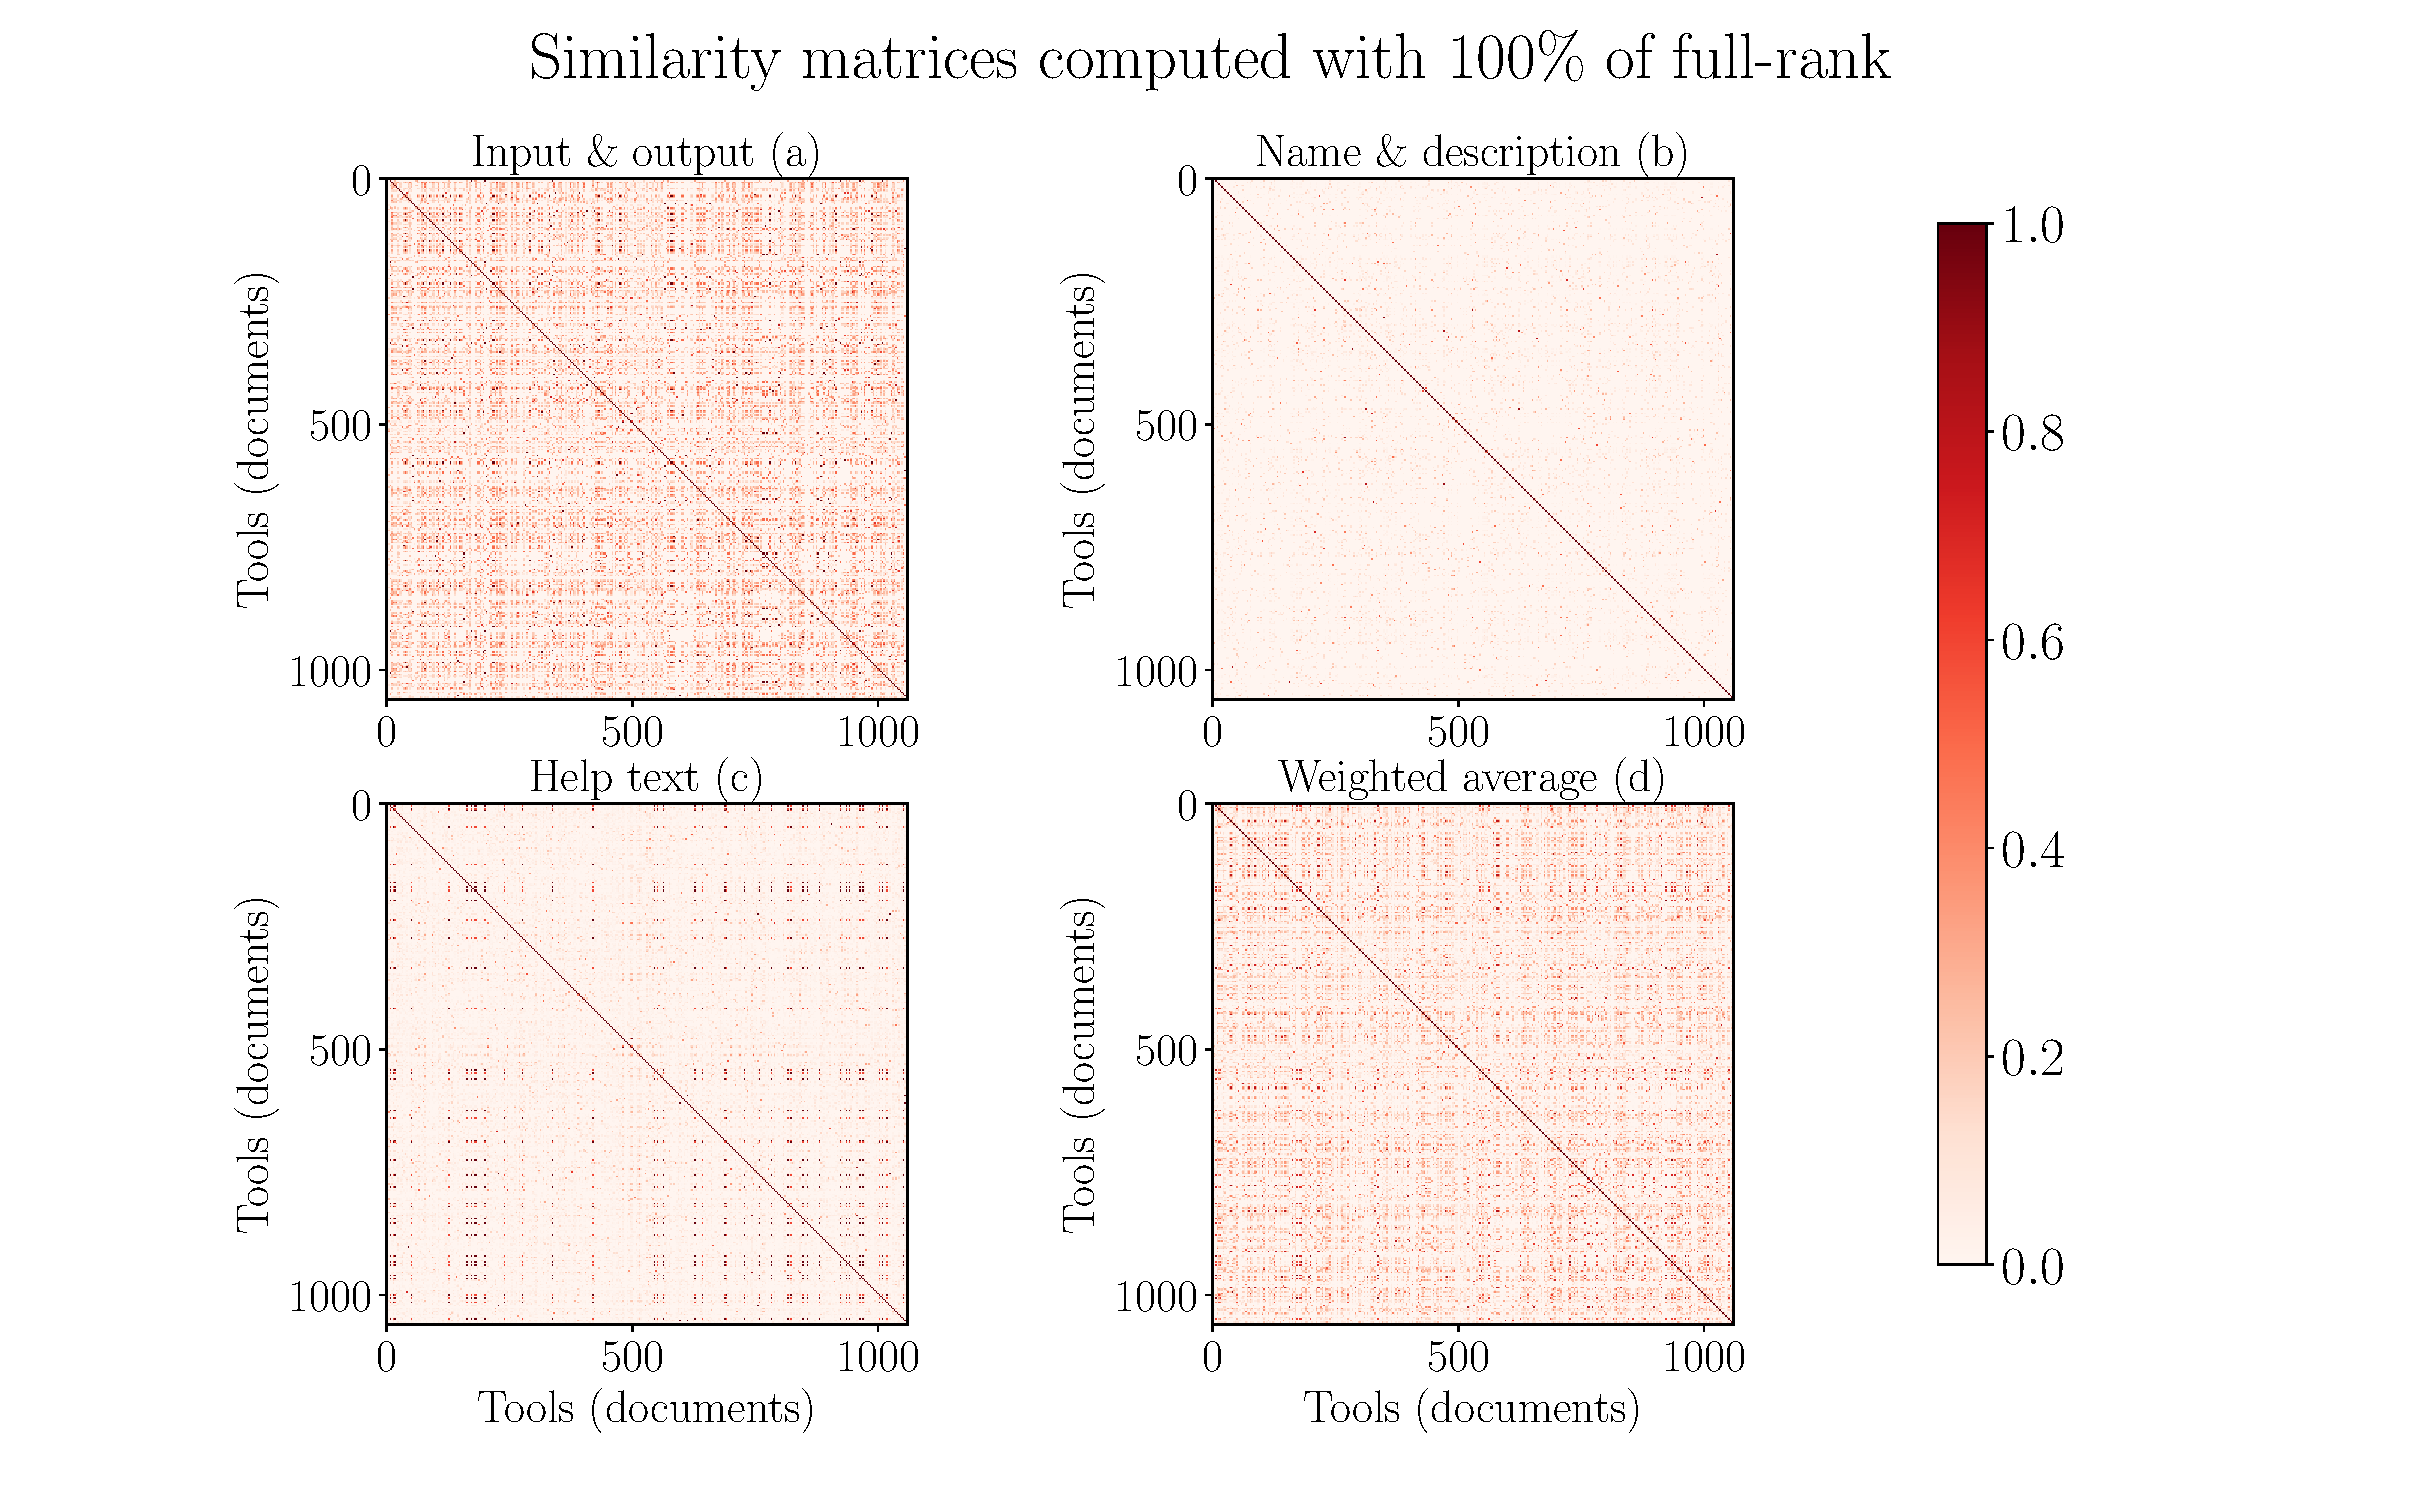
\includegraphics[scale=0.35]{figures/Similarity_matrices_100.pdf}}
    \caption[Similarity matrices full rank]{\textbf{Similarity matrices using full-rank}: The heatmap shows documents-documents (tools-tools) correlation matrices for input and output (a), name and description (b) and help text (c) attributes. The (d) shows a documents-documents (tools-tools) correlation matrix which is the weighted average computed using (a), (b) and (c) and weights (figure 18) given by the gradient descent optimizer (equation 15). The corresponding documents-tokens matrices contain their full-ranks. }
\end{centering}
\end{figure}

\begin{figure}[h]
\begin{centering}
    {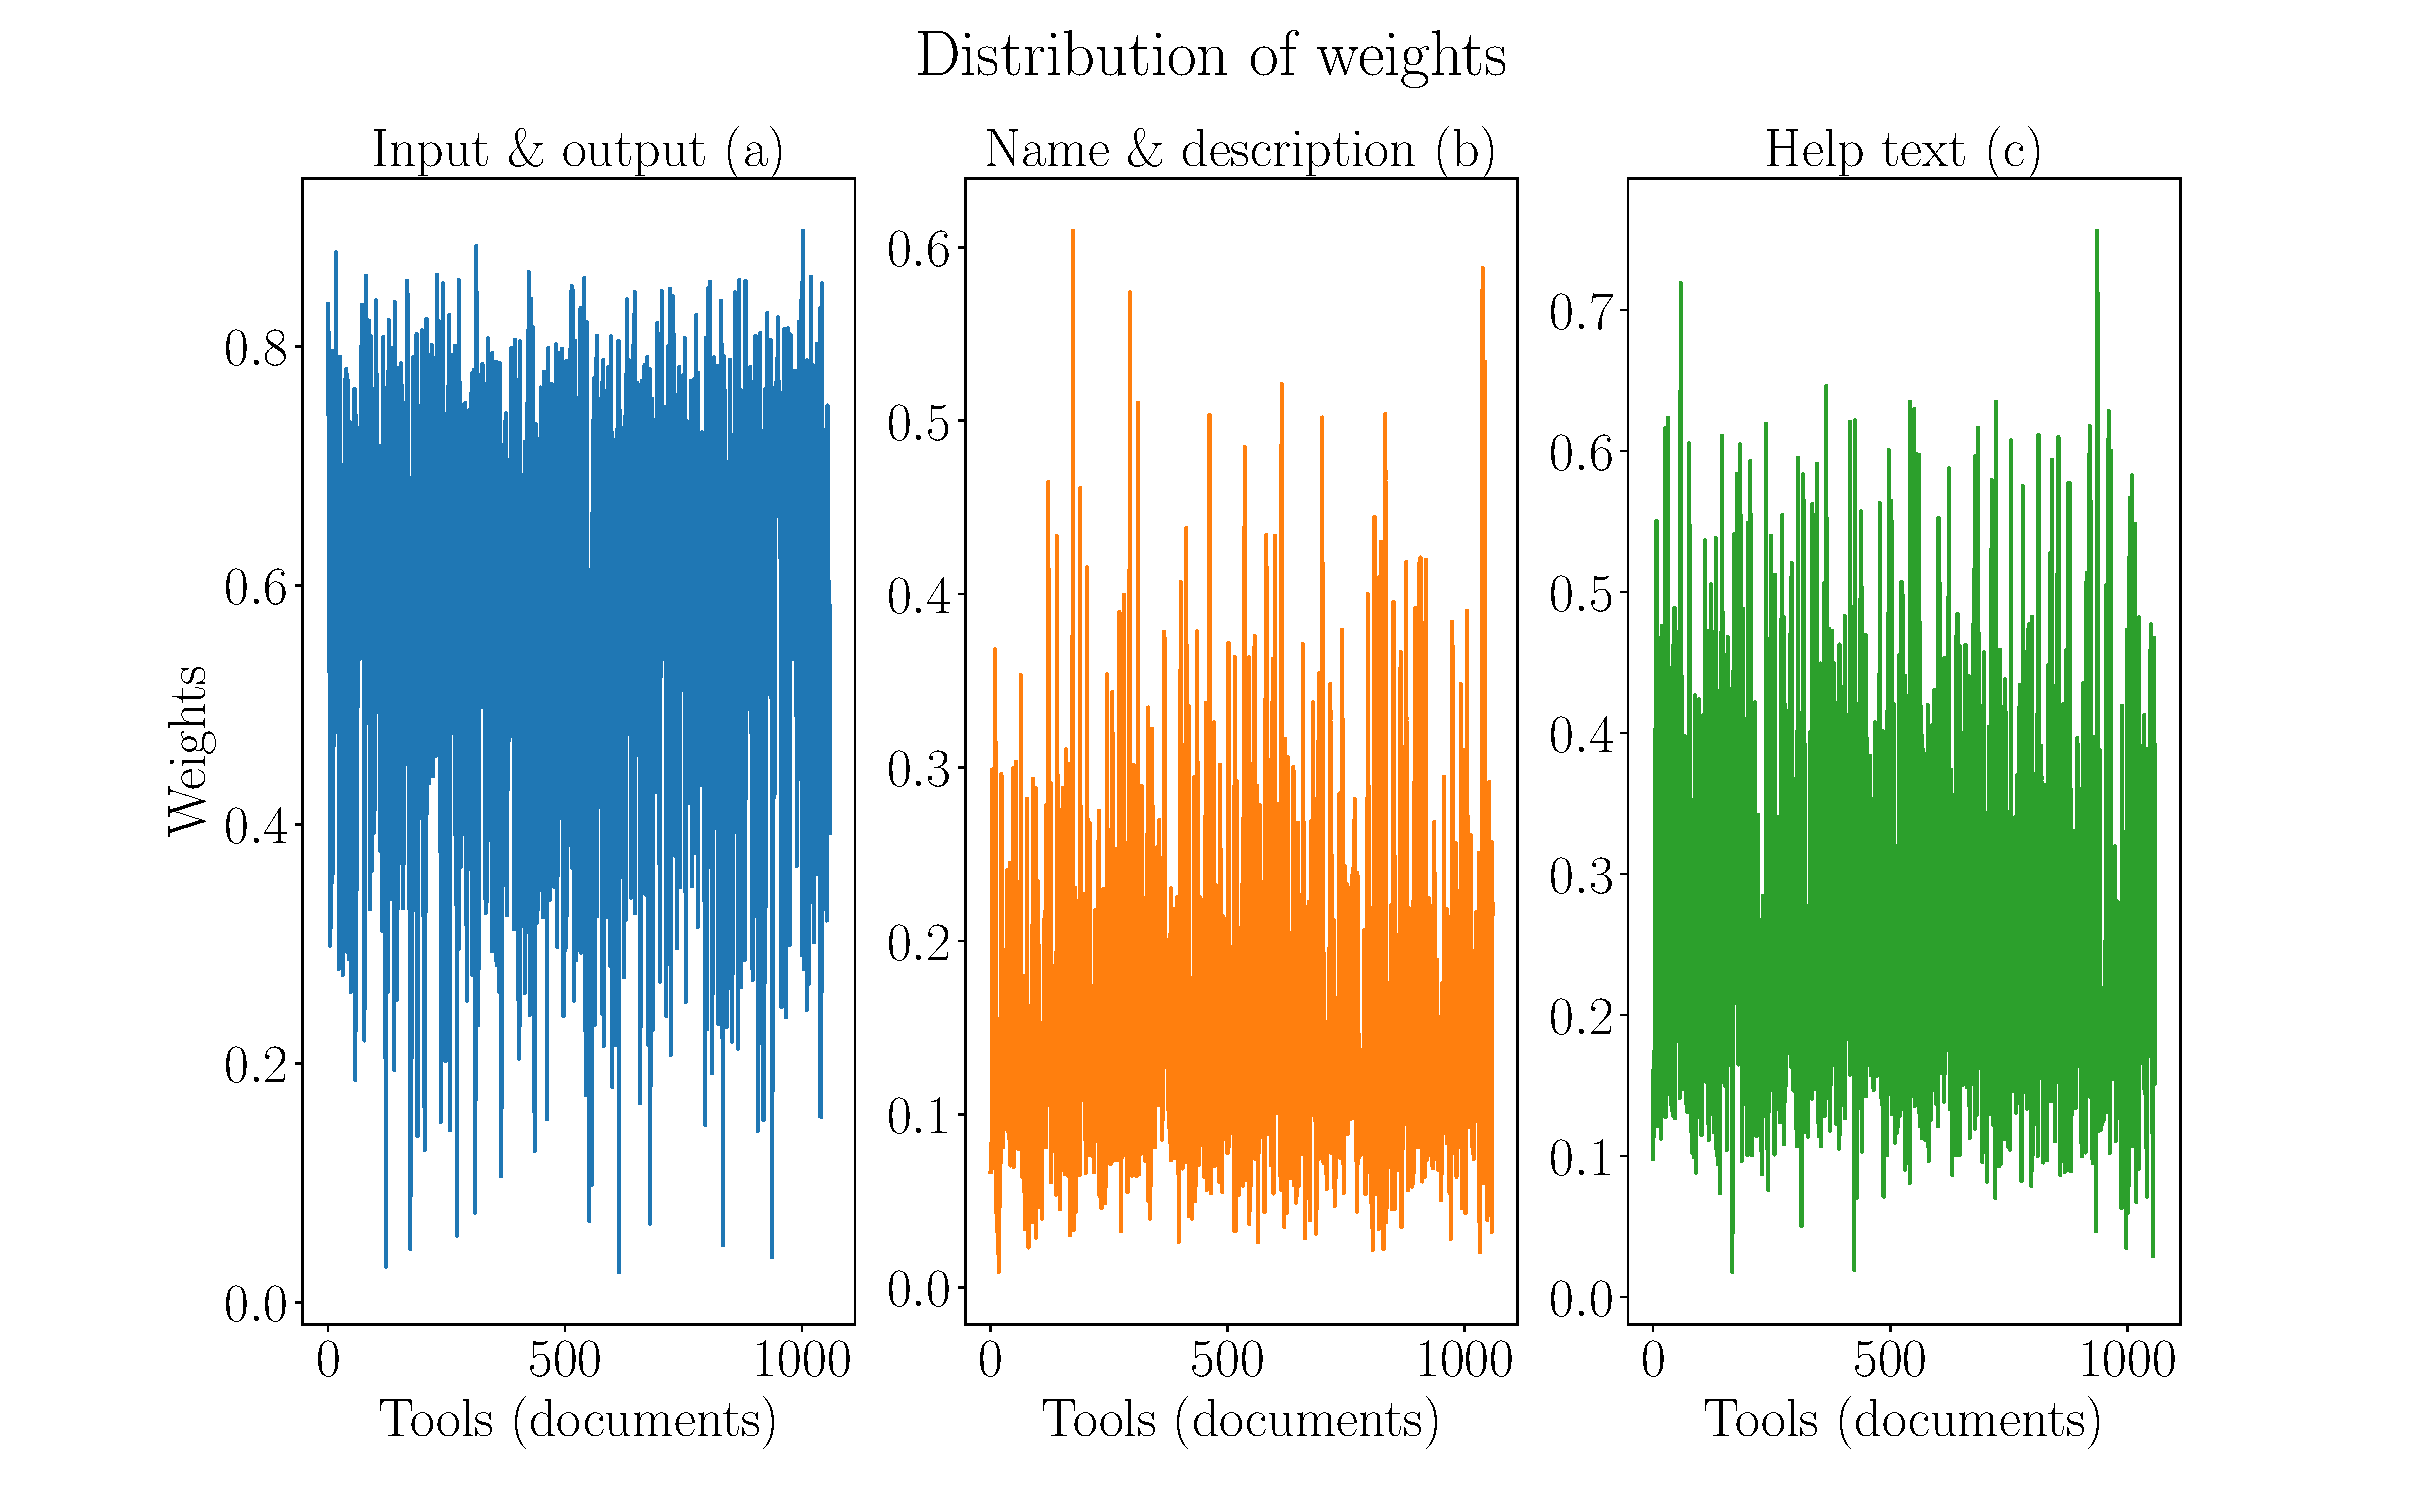
\includegraphics[scale=0.35]{figures/Weights_100.pdf}}
    \caption[Weights distribution full-rank]{\textbf{Weights distribution full- rank}: The plot shows the distribution of weights learned by gradient descent optimizer on the similarity matrices for the input and output, name and description and help text attributes. The corresponding documents-tokens matrices contain their full-ranks.}
\end{centering}
\end{figure}

\subsection{70\% of full-rank}
In figure 17, we can see that the similarity matrices for name and description and help text are sparse. To reduce the sparsity,  we attempt to reduce the ranks of the respective documents-tokens matrices of these two attributes to 70\% of full-rank. For example, if the rank of a matrix is 100, we reduce the rank to 70 using singular value decomposition. Along with reducing the ranks, we reduce the singular values of these matrices as well. Comparing figures 17 and 19, we see that the name and description and help text similarity matrices start becoming more dense. The distribution of the weights also change (figures 18 and 20). At this stage, it is hard to see the effect of rank reduction. Further we reduce the ranks drastically to see the effect.

\begin{figure}[h]
\begin{centering}
    {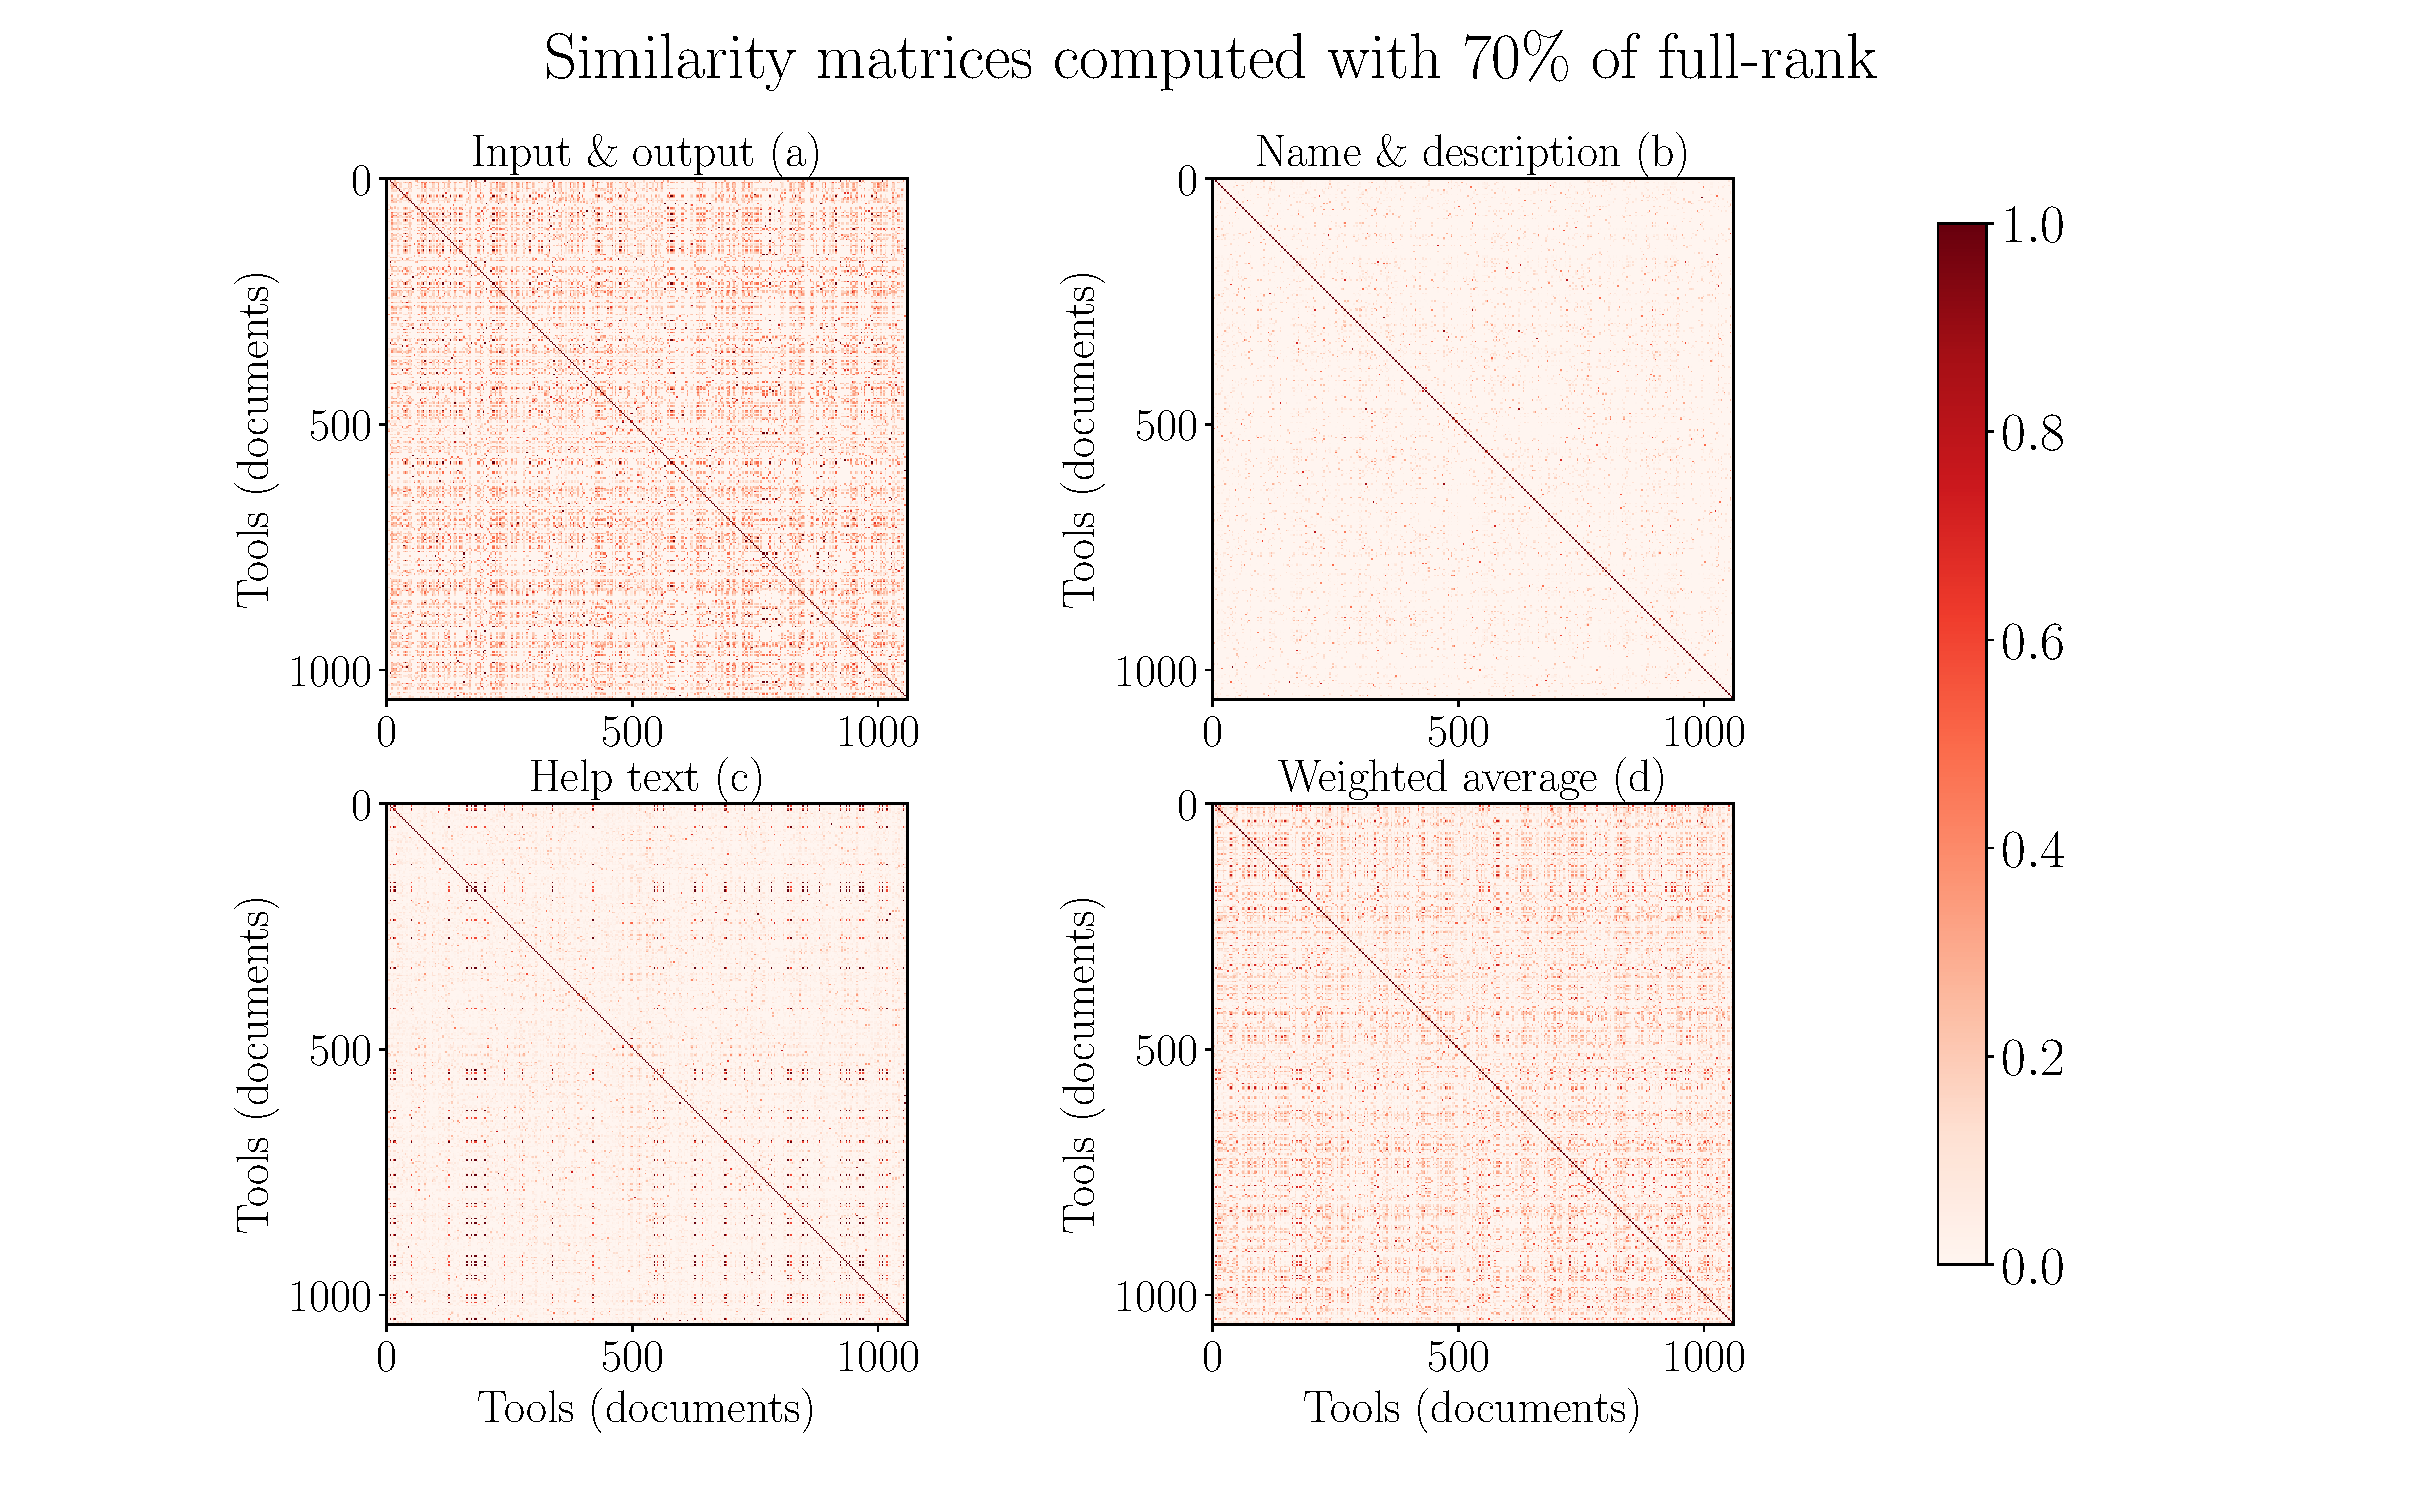
\includegraphics[scale=0.35]{figures/Similarity_matrices_070.pdf}}
    \caption[Similarity matrices 70\% rank]{\textbf{Similarity matrices using 70\% of full-rank}: The heatmap shows documents-documents (tools-tools) correlation matrices for input and output (a), name and description (b) and help text (c) attributes. The (d) shows a documents-documents (tools-tools) correlation matrix which is the weighted average computed using (a), (b) and (c) and weights (figure 20) given by the gradient descent optimizer (equation 15). The corresponding documents-tokens matrices are reduced to 70\% of their respective full-ranks.}
\end{centering}
\end{figure}

\begin{figure}[h]
\begin{centering}
    {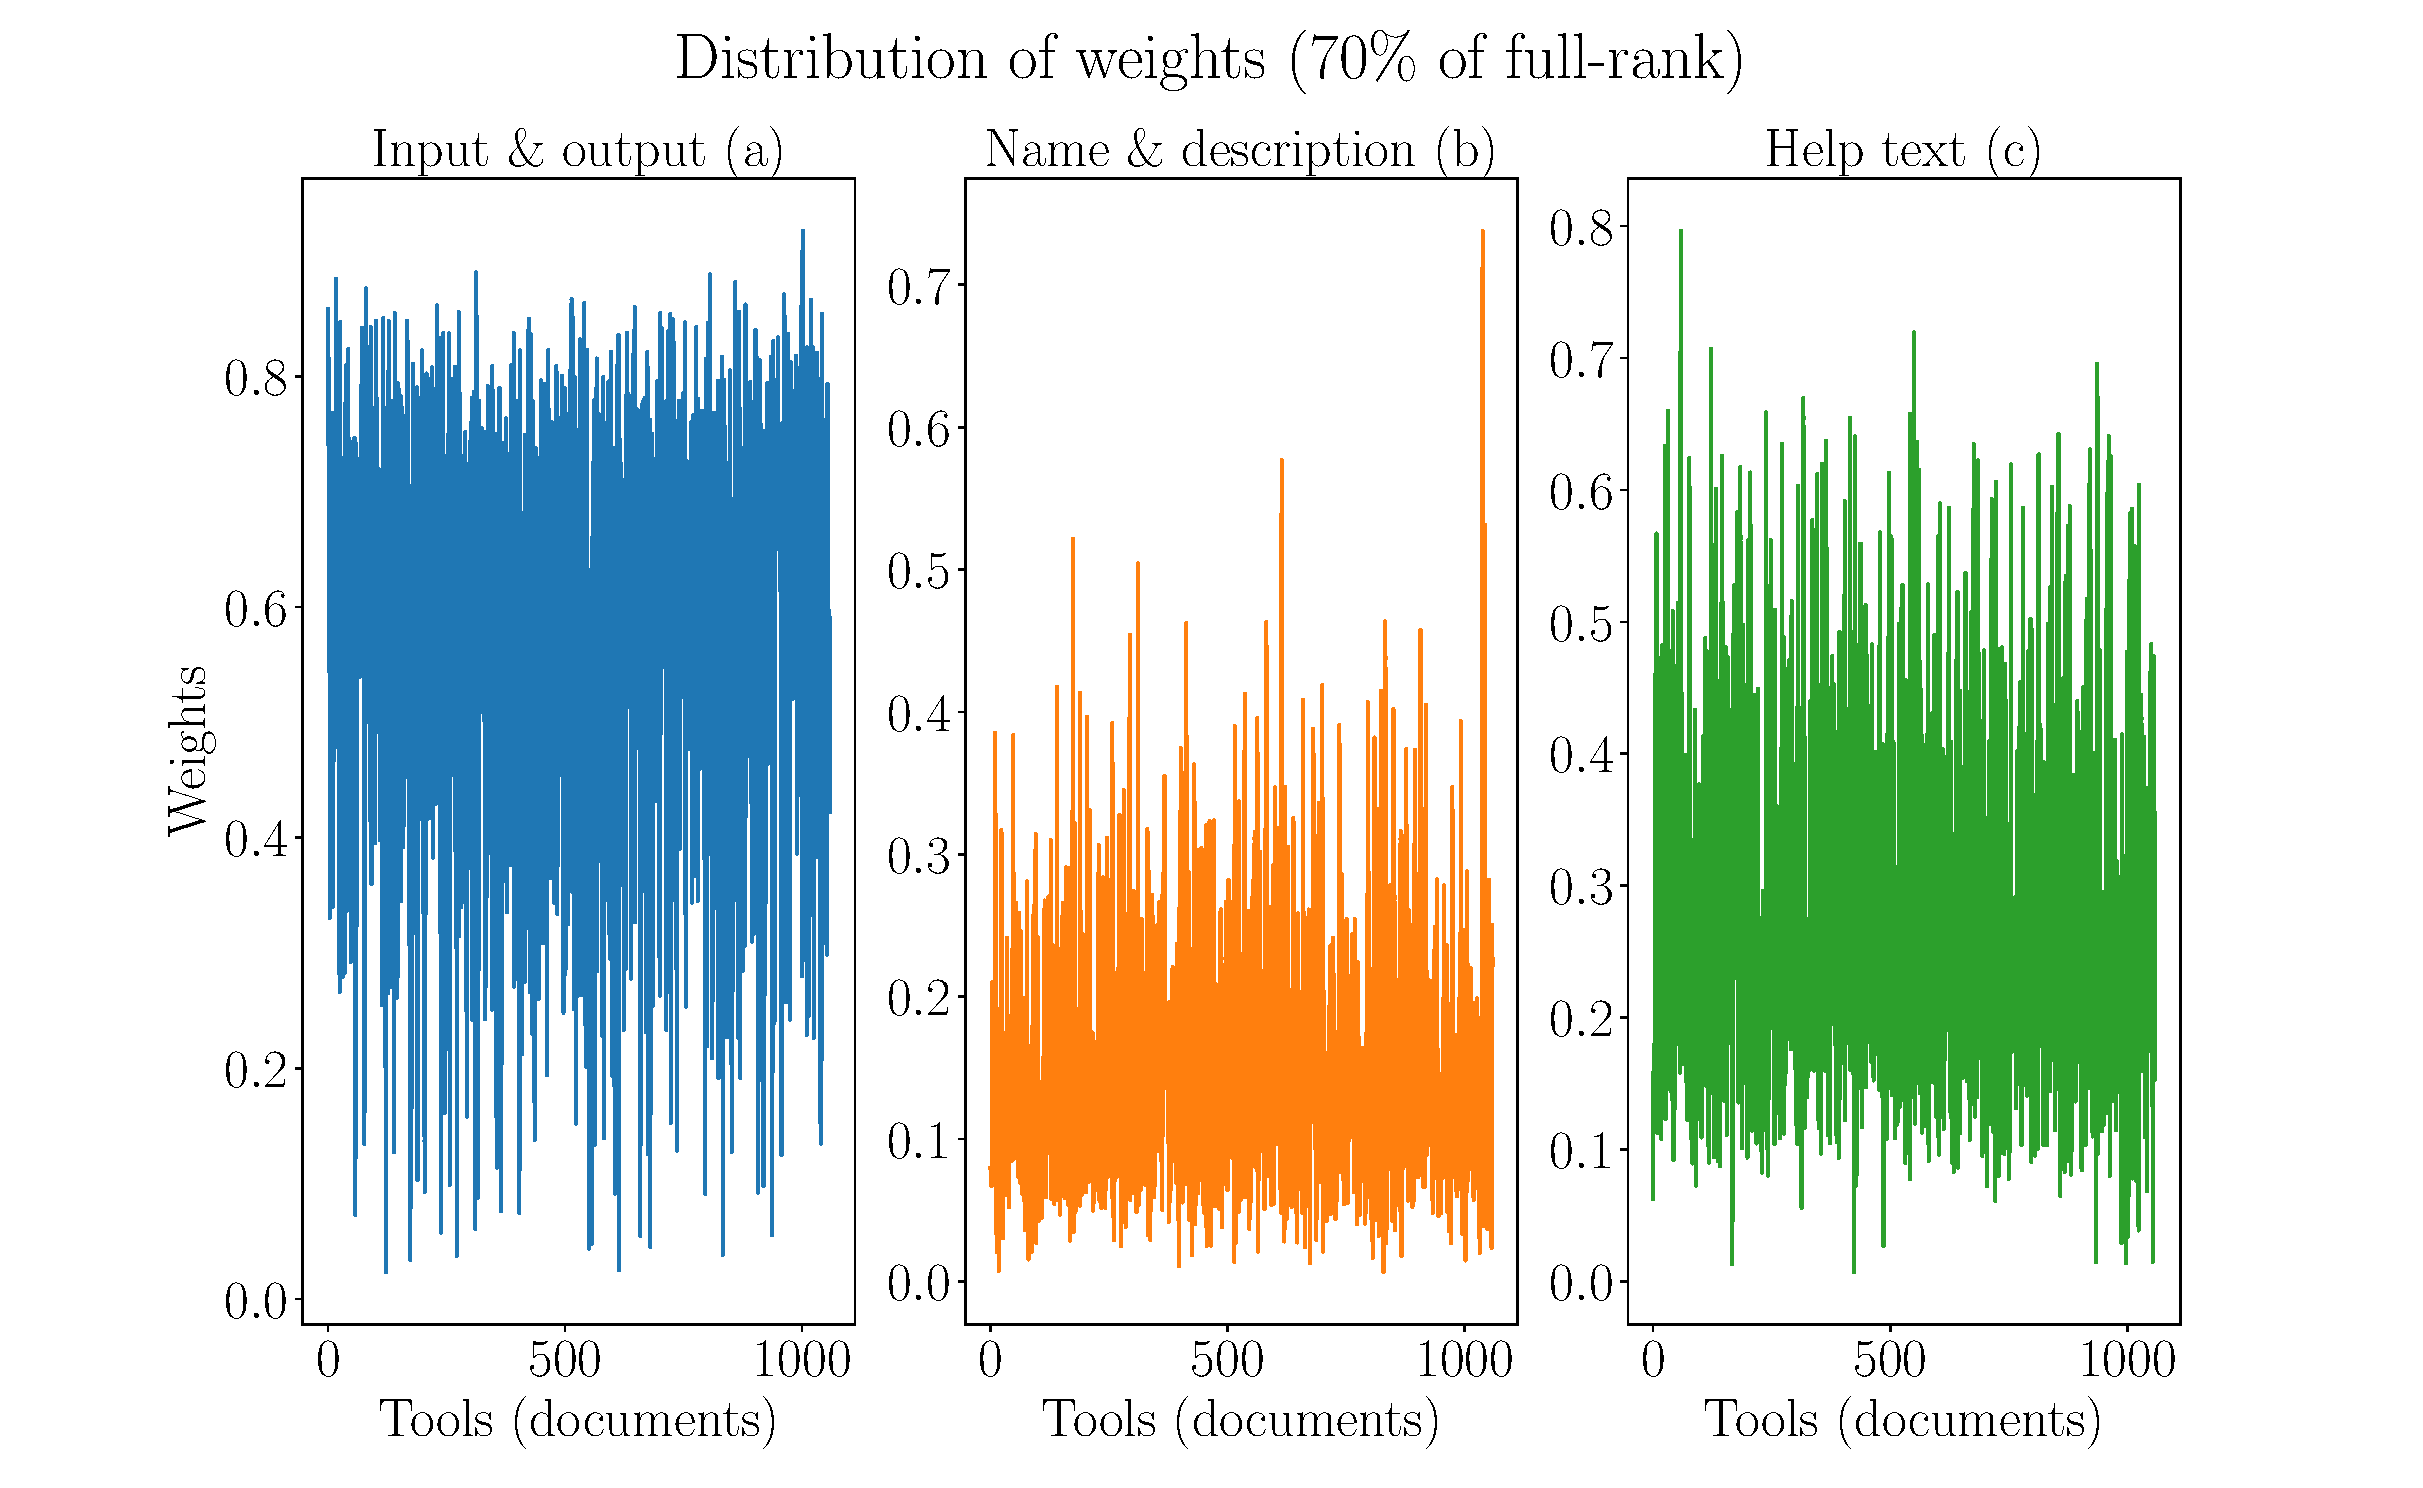
\includegraphics[scale=0.35]{figures/Weights_070.pdf}}
    \caption[Weights distribution 70\% rank]{\textbf{Weights distribution using 70\% of full-rank}: The plot shows the distribution of weights learned by gradient descent optimizer on the similarity matrices for the input and output, name and description and help text attributes. The corresponding documents-tokens matrices contain 70\% of their full-ranks.}
\end{centering}
\end{figure}

\subsection{30\% of full-rank}
To see the effect of rank reduction, we reduce the ranks of two documents-tokens matrices to 30\% of full-rank. This is a large reduction and would amount to keeping $\approx 60\%$ (removing $\approx 40\%$) (figure 11) of sum of singular values for all the documents-tokens matrices. In figures 21 and 22, the effect of rank reduction is more visible compared to $70\%$. We see that the magnitudes of weights learned for input and output files start to decrease and the magnitudes of weights for name and description and help text start to increase because the corresponding similarity matrices score become more dense (figure 21). 

\begin{figure}[h]
\begin{centering}
    {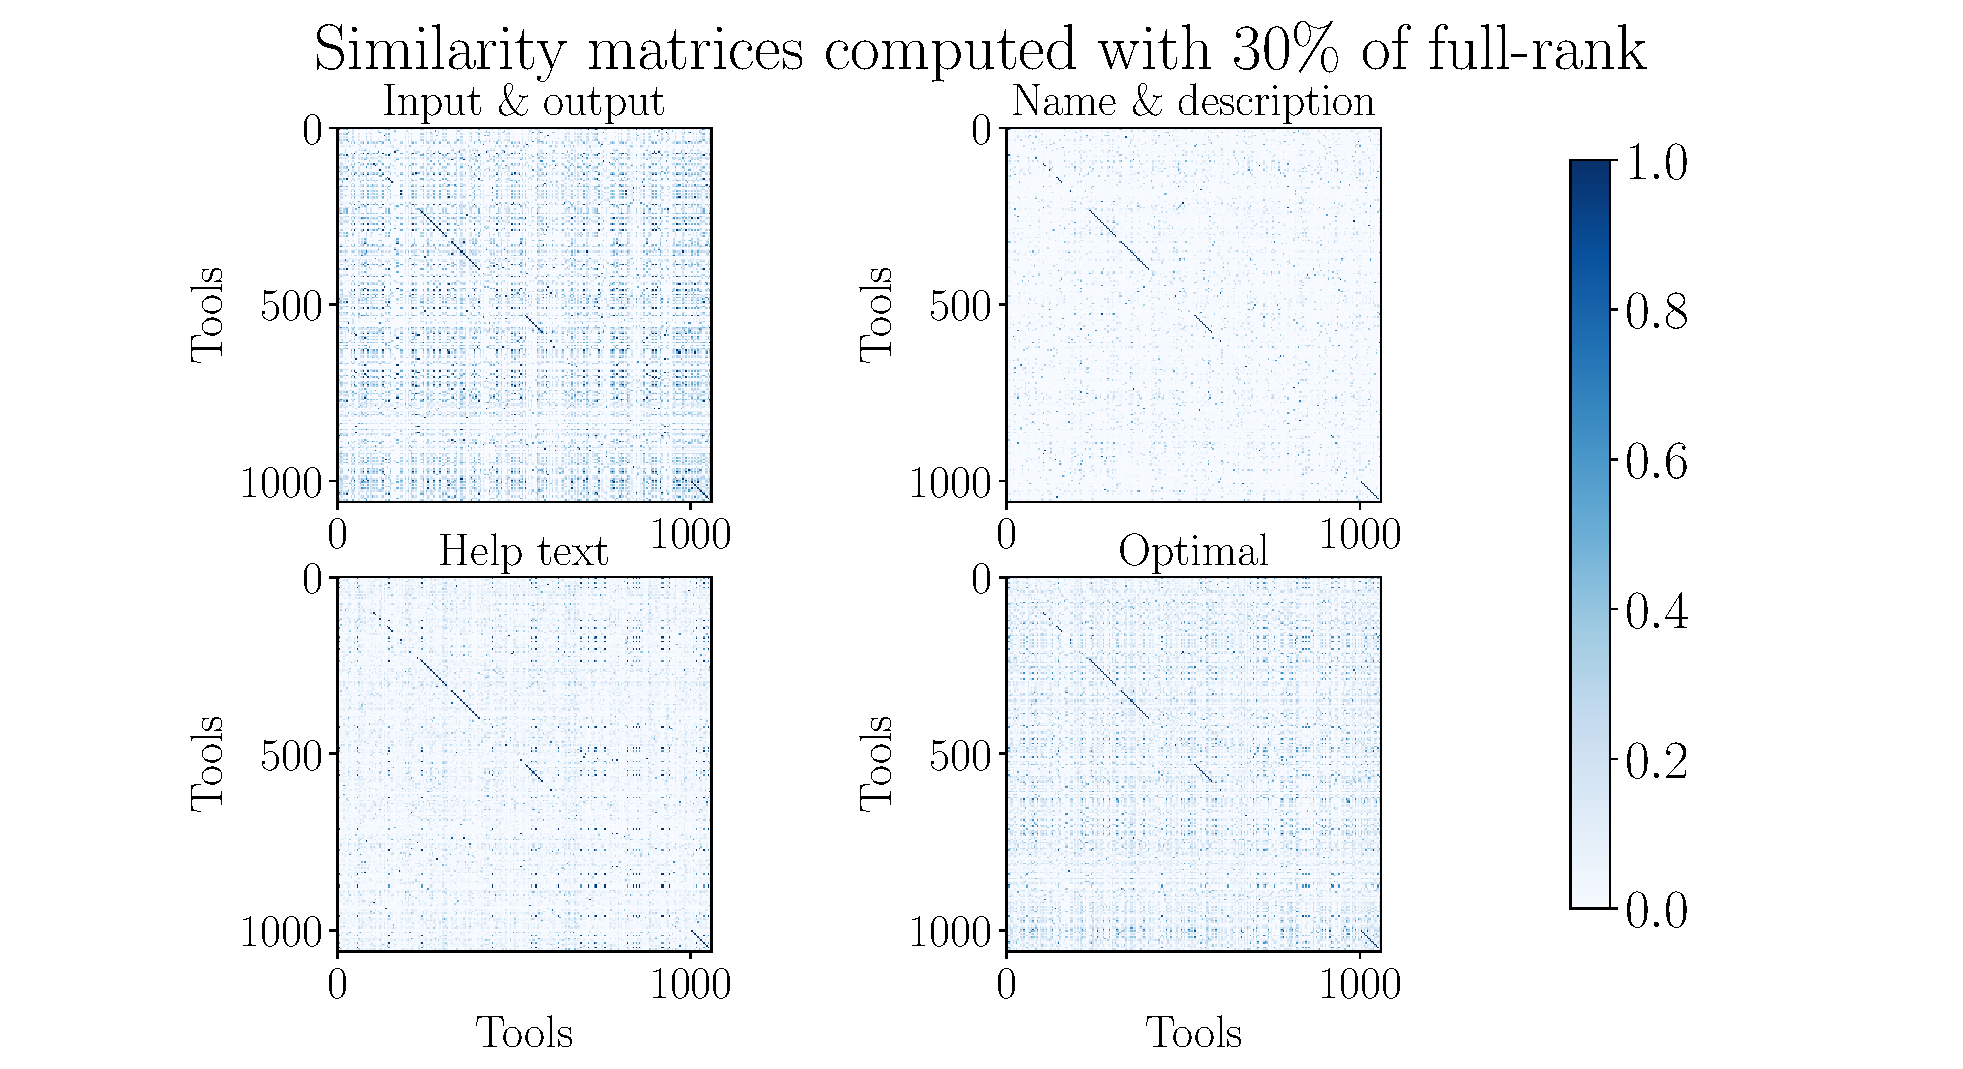
\includegraphics[scale=0.35]{figures/Similarity_matrices_030.pdf}}
    \caption[Similarity matrices 30\% rank]{\textbf{Similarity matrices using 30\% of full-rank}: The heatmap shows documents-documents (tools-tools) correlation matrices for input and output (a), name and description (b) and help text (c) attributes. The (d) shows a documents-documents (tools-tools) correlation matrix which is the weighted average computed using (a), (b) and (c) and weights (figure 22) given by the gradient descent optimizer (equation 15). The corresponding documents-tokens matrices are reduced to 30\% of their respective full-ranks.}
\end{centering}
\end{figure}

\begin{figure}[h]
\begin{centering}
    {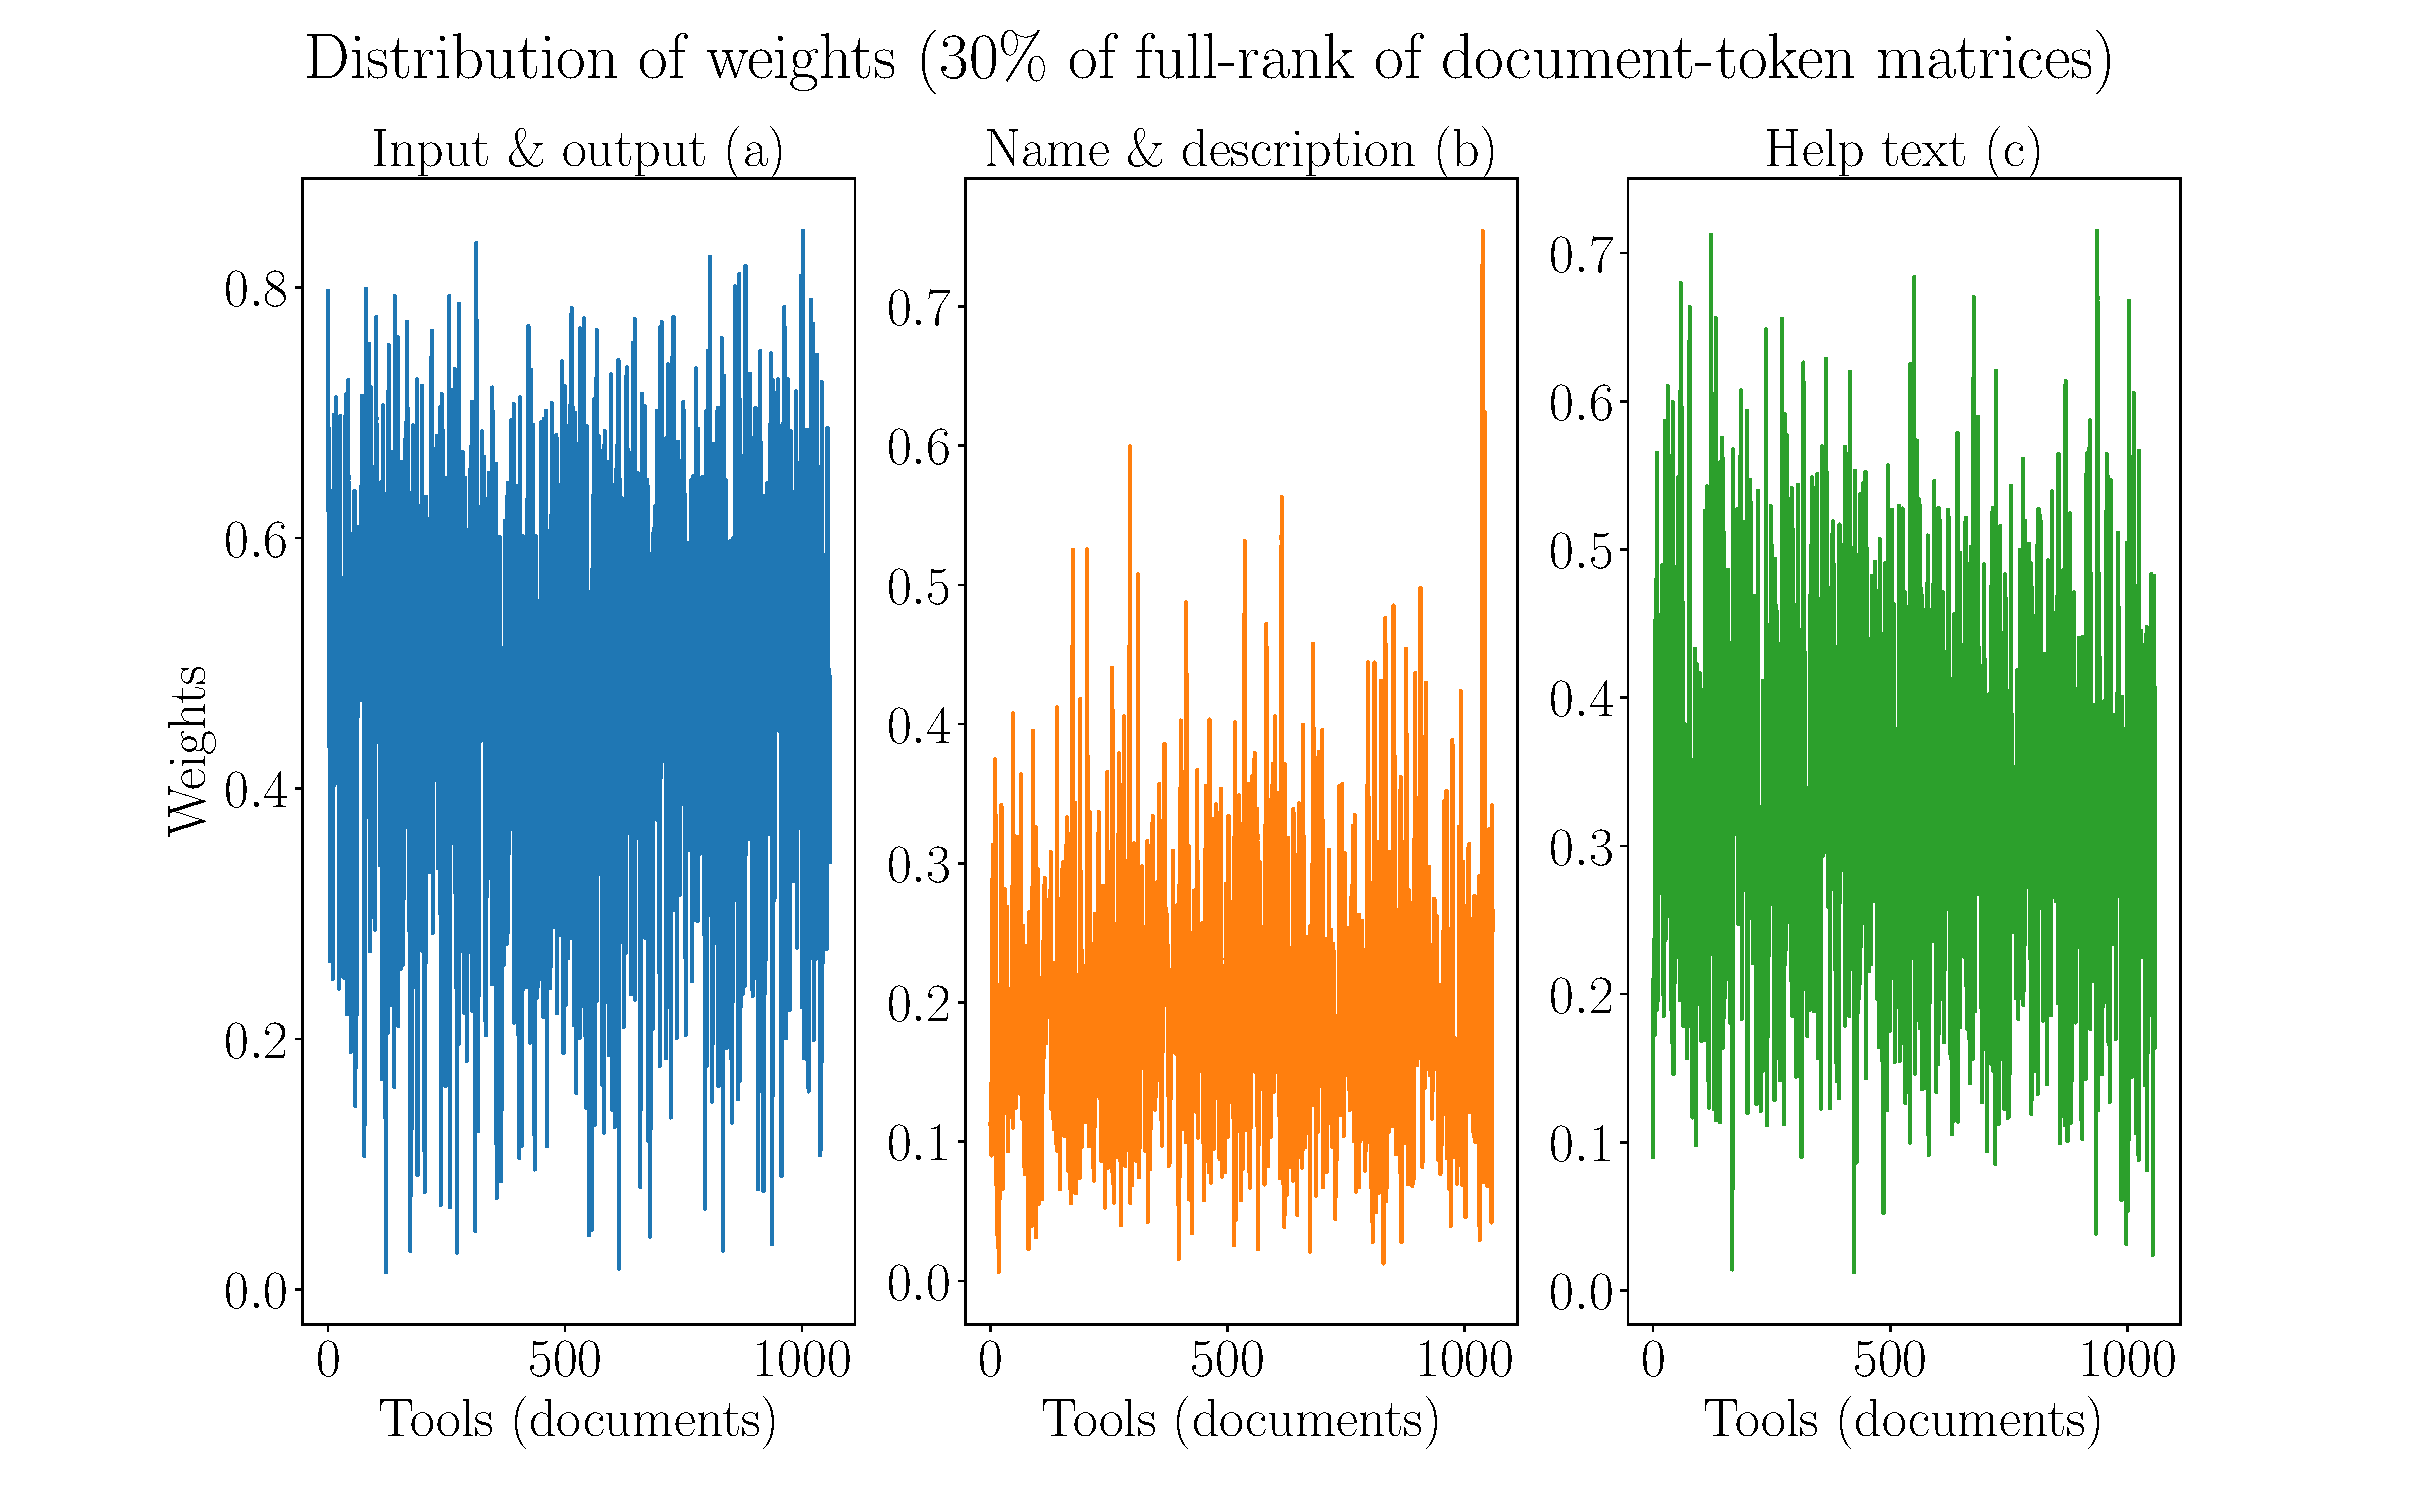
\includegraphics[scale=0.35]{figures/Weights_030.pdf}}
    \caption[Weights distribution 30\% rank]{\textbf{Weights distribution using 30\% of full-rank}: The plot shows the distribution of weights learned by gradient descent optimizer on the similarity matrices for the input and output, name and description and help text attributes. The corresponding documents-tokens matrices contain 30\% of their full-ranks.}
\end{centering}
\end{figure}

\subsection{5\% of full-rank}
To verify the reduction in sparsity, we reduce the ranks of two documents-tokens matrices to 5\% of the full-rank. By choosing this low value, we consider only top $\approx 20\%$ of the sum of singular values for all the attributes (figure 11). From figure 23, we can see that all the similarity matrices corresponding to the attributes become more dense compared to figure 17, 91 and 21. Due to this, the weights distribution also change (figure 24). We learn higher weights for name and description (24b) and help text (24c). Along side, the weights on the input and output file types decrease (24a).  

\begin{figure}[h]
\begin{centering}
    {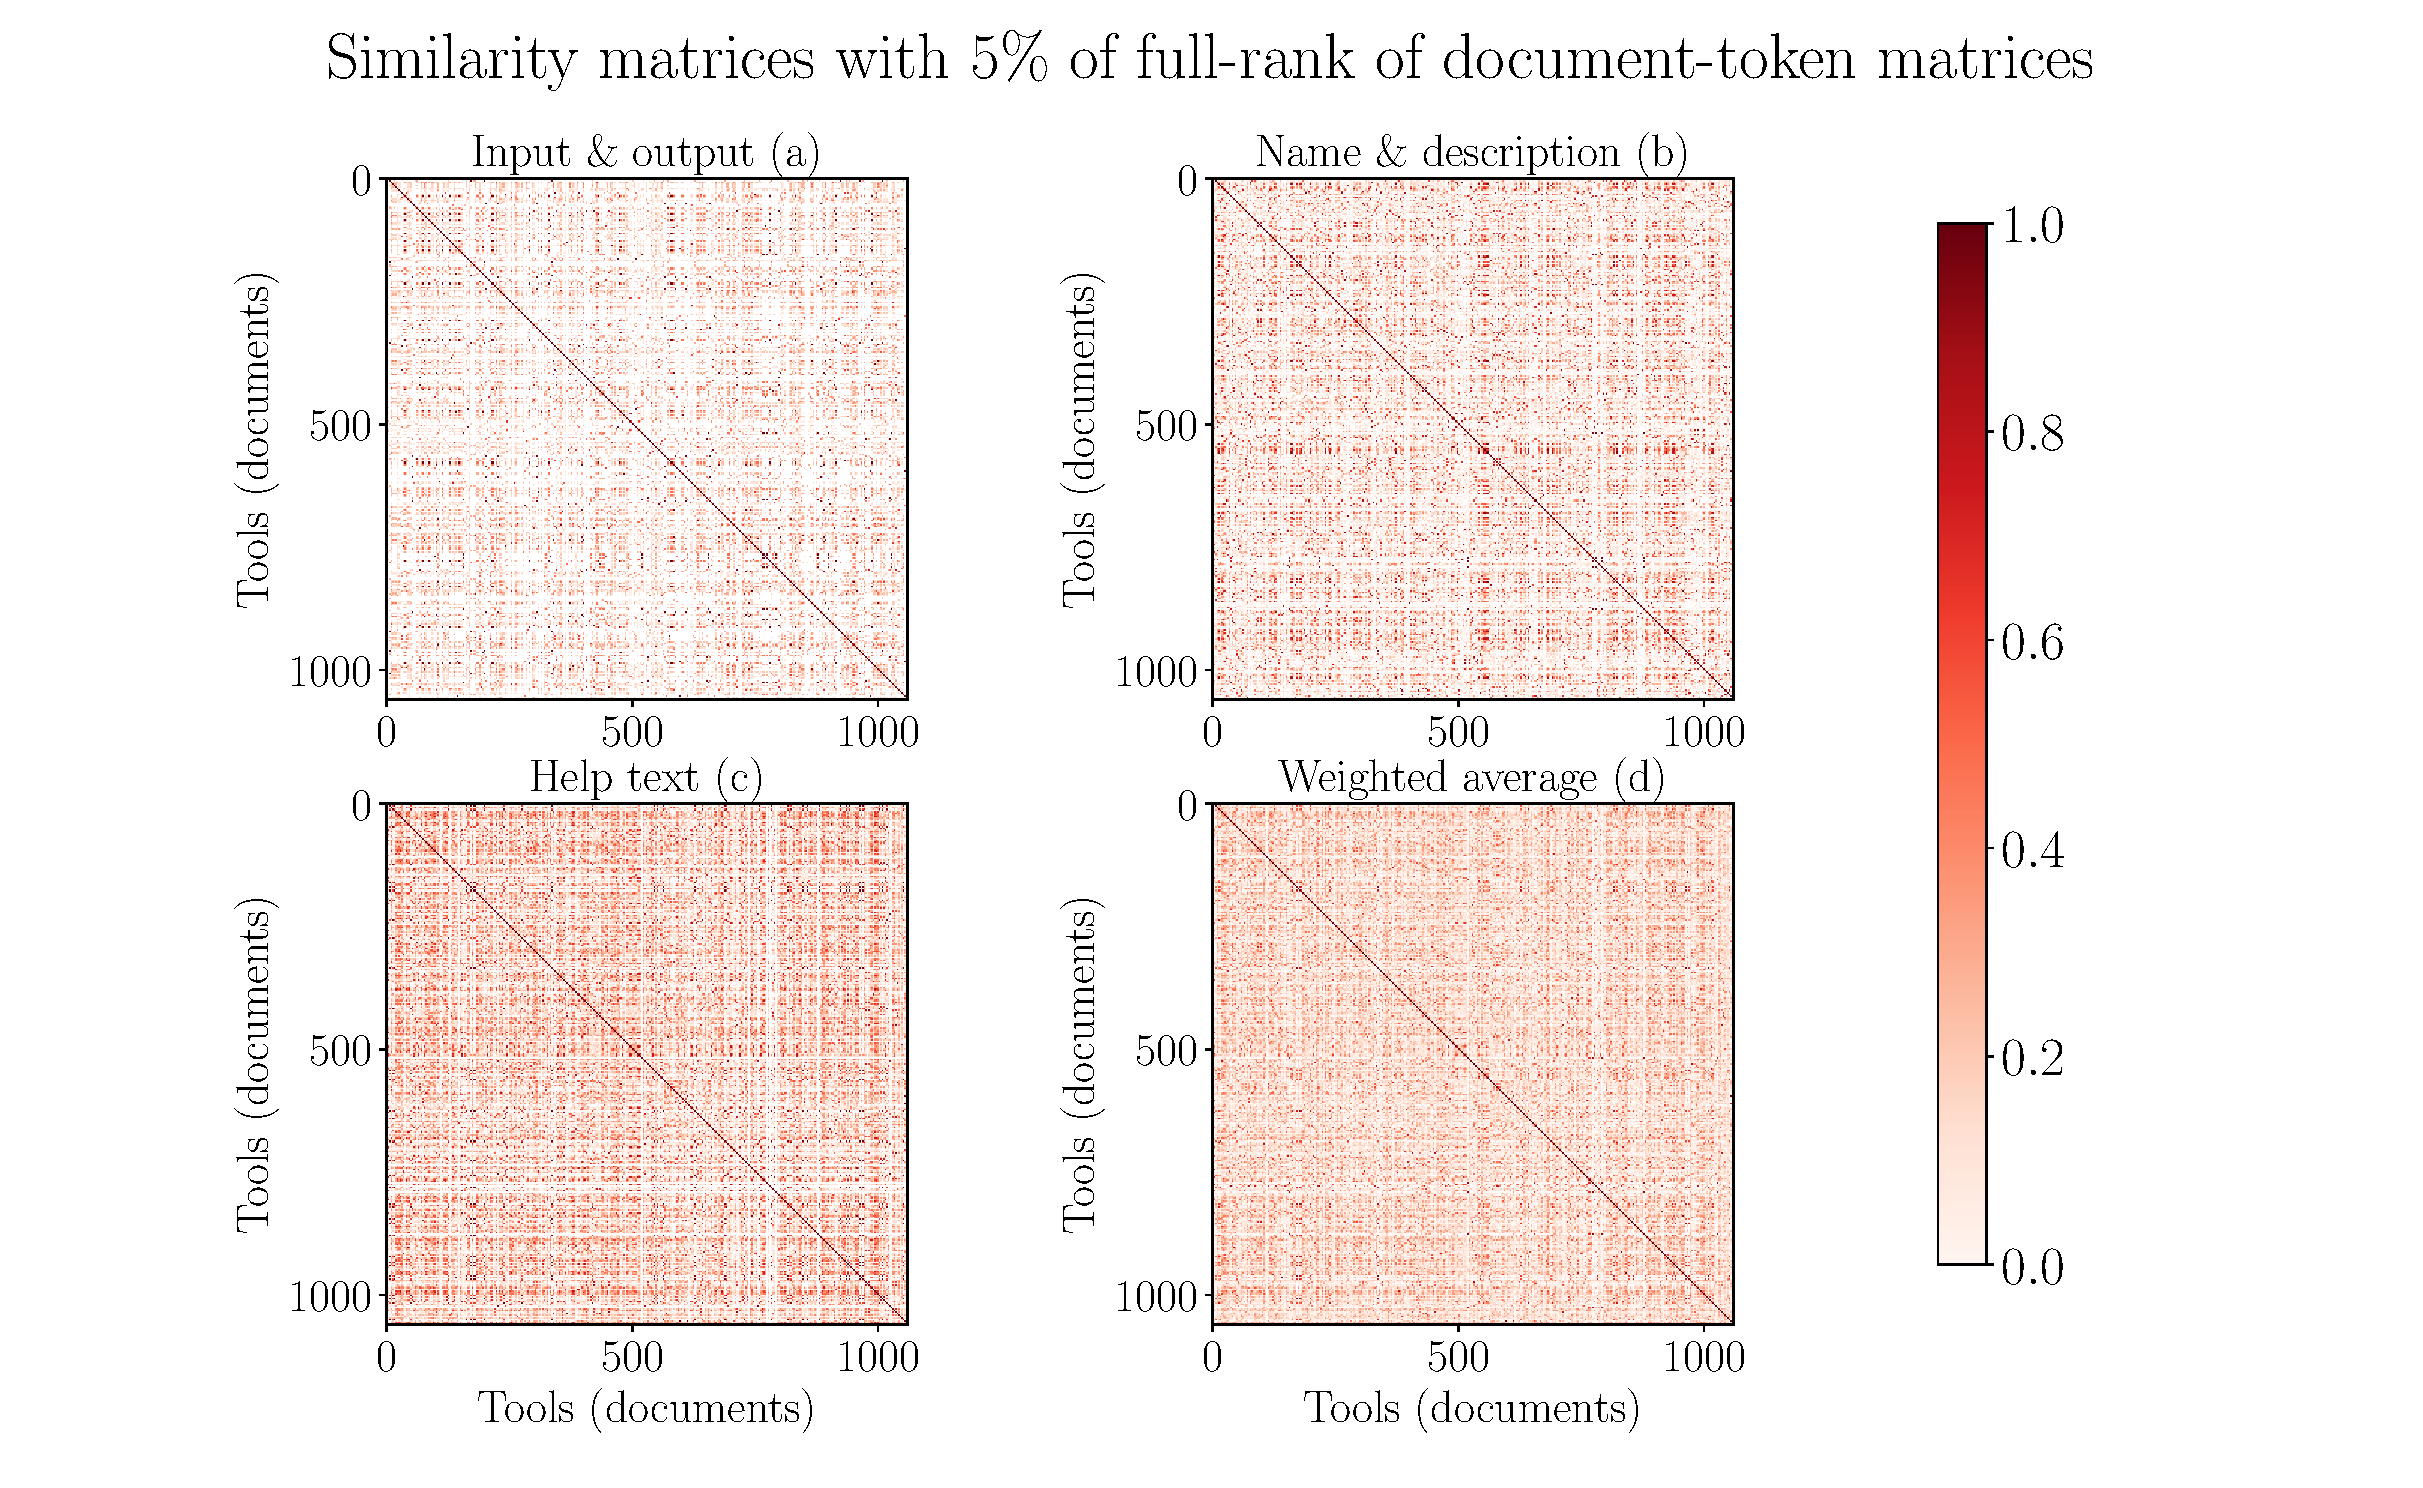
\includegraphics[scale=0.35]{figures/Similarity_matrices_005.pdf}}
    \caption[Similarity matrices 5\% rank]{\textbf{Similarity matrices using 5\% of full-rank}: The heatmap shows documents-documents (tools-tools) correlation matrices for input and output (a), name and description (b) and help text (c) attributes. The (d) shows a documents-documents (tools-tools) correlation matrix which is the weighted average computed using (a), (b) and (c) and weights (figure 24) given by the gradient descent optimizer (equation 15). The corresponding documents-tokens matrices are reduced to 5\% of their respective full-ranks.}
\end{centering}
\end{figure}

\begin{figure}[h]
\begin{centering}
    {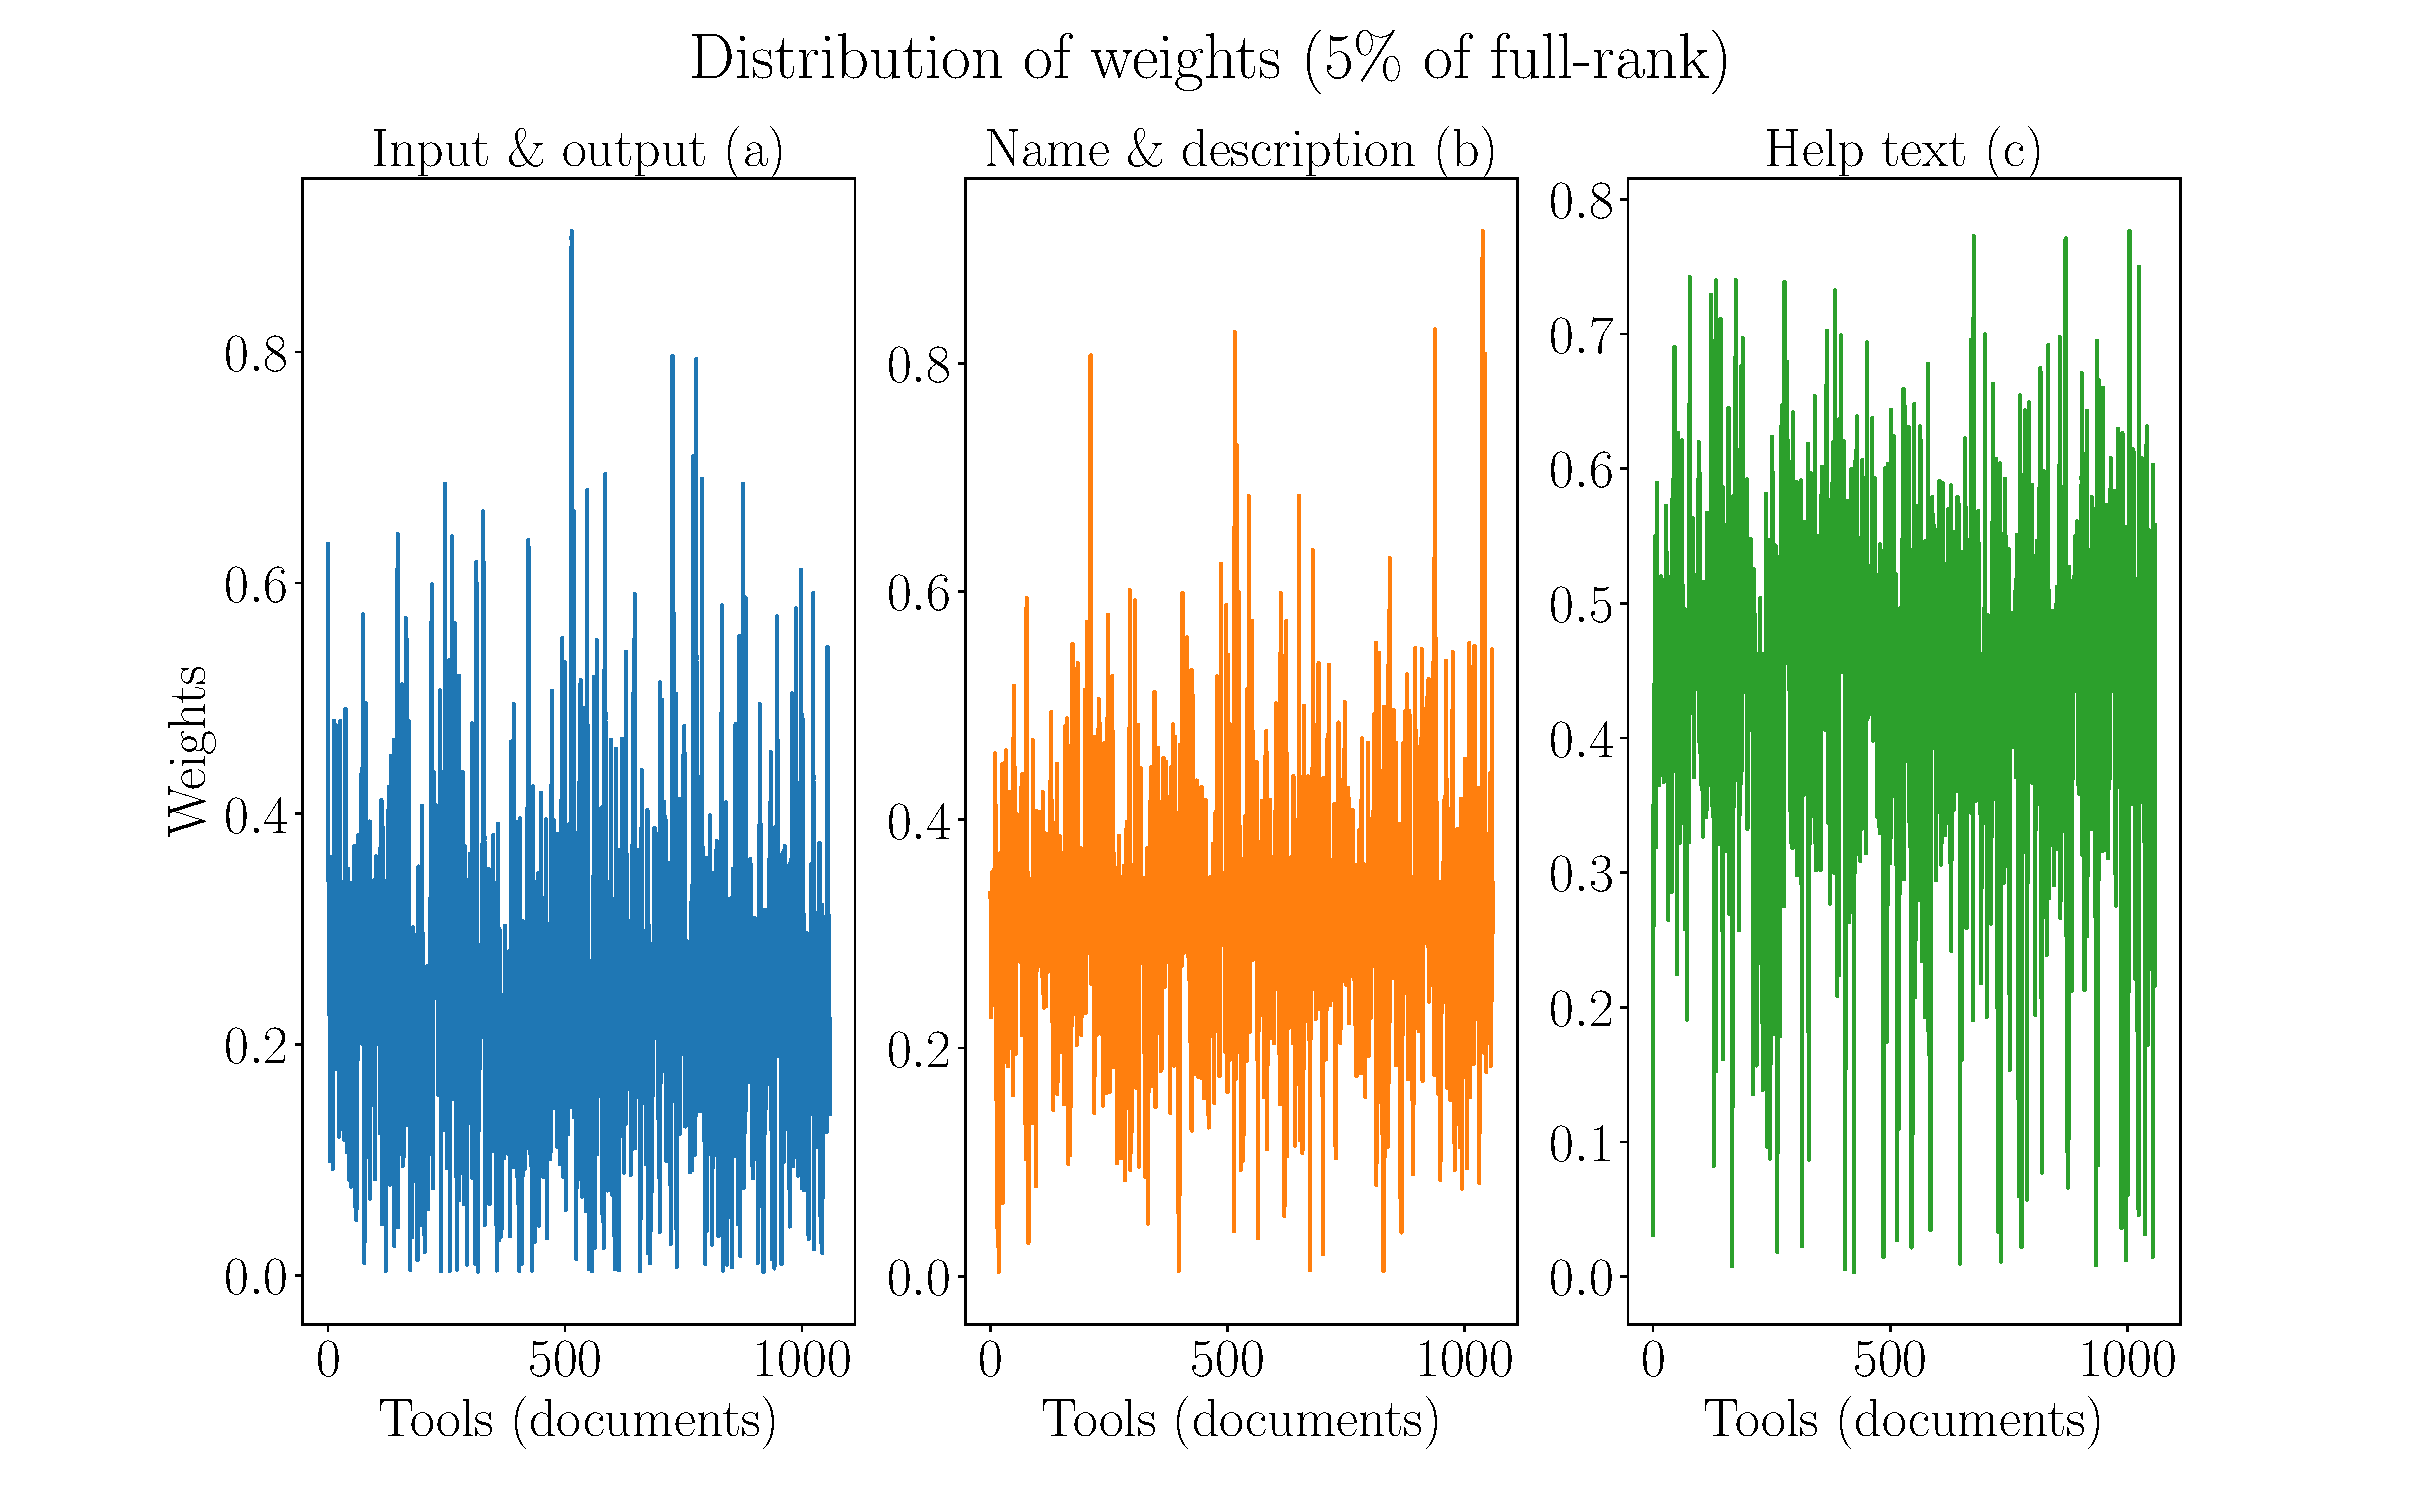
\includegraphics[scale=0.35]{figures/Weights_005.pdf}}
    \caption[Weights distribution 5\% rank]{\textbf{Weights distribution using 5\% of full-rank}: The plot shows the distribution of weights learned by gradient descent optimizer on the similarity matrices for the input and output, name and description and help text attributes. The corresponding documents-tokens matrices contain 5\% of their full-ranks.}
\end{centering}
\end{figure}

\subsection{Improvement verification}
To verify that the matrix rank reduction actually works and learns better similarity scores for tools (documents) which are similar in actual case, we showcase two ways.

\subsubsection{Reduction in error}
We observe drop in mean squared error when we decrease the ranks of the matrices. When we reduce the ranks, the similarity scores for the name and description and help text increase. This increase accounts for their larger weights learned by the optimizer. The weights on an average become more balanced and together with higher similarity scores account for the decrease in the mean squared error. In the absence of true similarity values, this viewpoint might not be completely correct way to establish that we actually improve the performance. To be more certain, we created a visualizer using javascript and html to look through the similar tools and their respective scores and weights for all tools. The next section explains it.

\subsubsection{Visualizer for latent semantic analysis approach}
% screenshots
We see the similar tools for a few selected tools for the different stage of rank reduction and verify if we actually fetch the similar tools.

\begin{figure}[h]
\begin{centering}
    {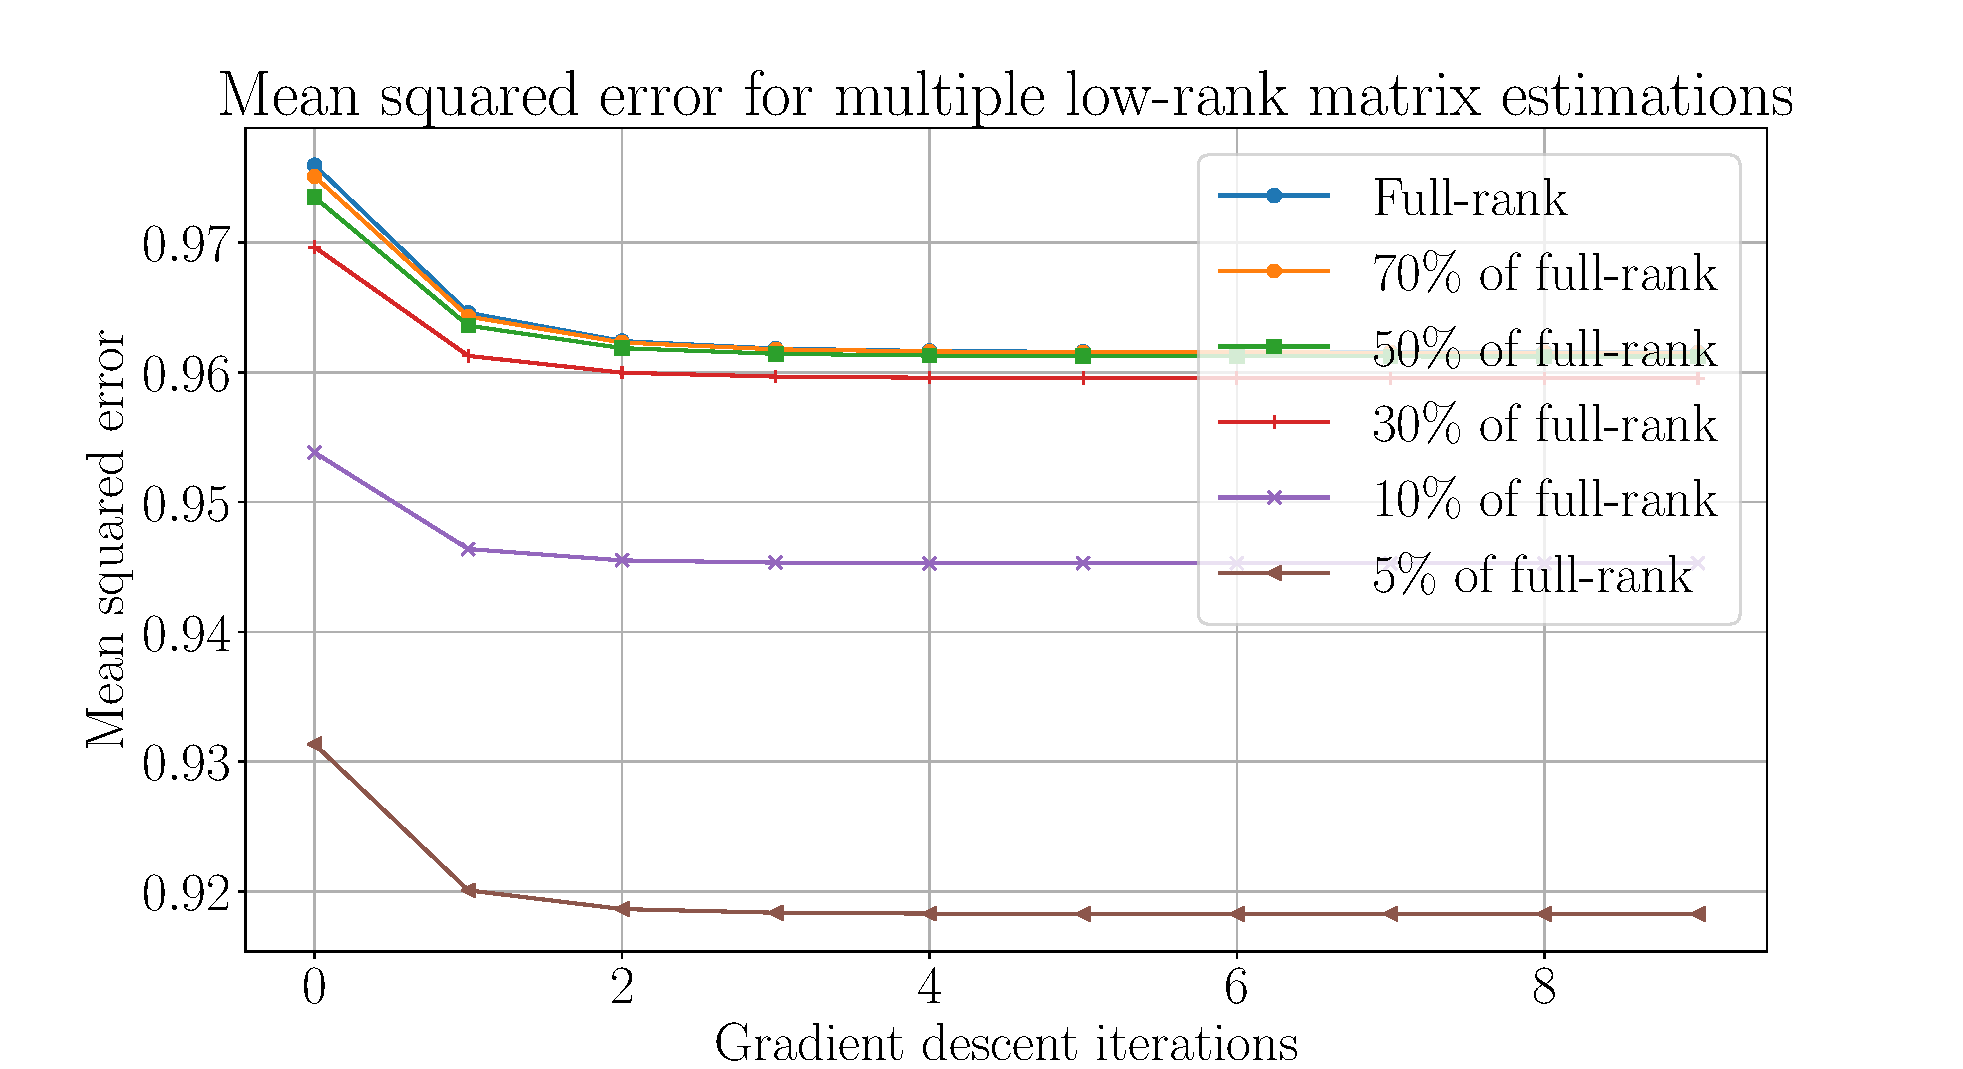
\includegraphics[scale=0.35]{figures/MSE_iterations_low_rank.pdf}}
    \caption[Mean squared error using LSI]{\textbf{Mean squared error using full-rank and multiple estimations of low-rank documents-tokens matrices}: This shows an mean squared error comparison computed using full-rank and various estimations of low-rank documents-tokens matrices. Each line plot shows an average error over all the tools and attributes which drops as we move along the iterations of gradient descent.}
\end{centering}
\end{figure}

\section{Paragraph vectors}

\begin{figure}[h]
\begin{centering}
    {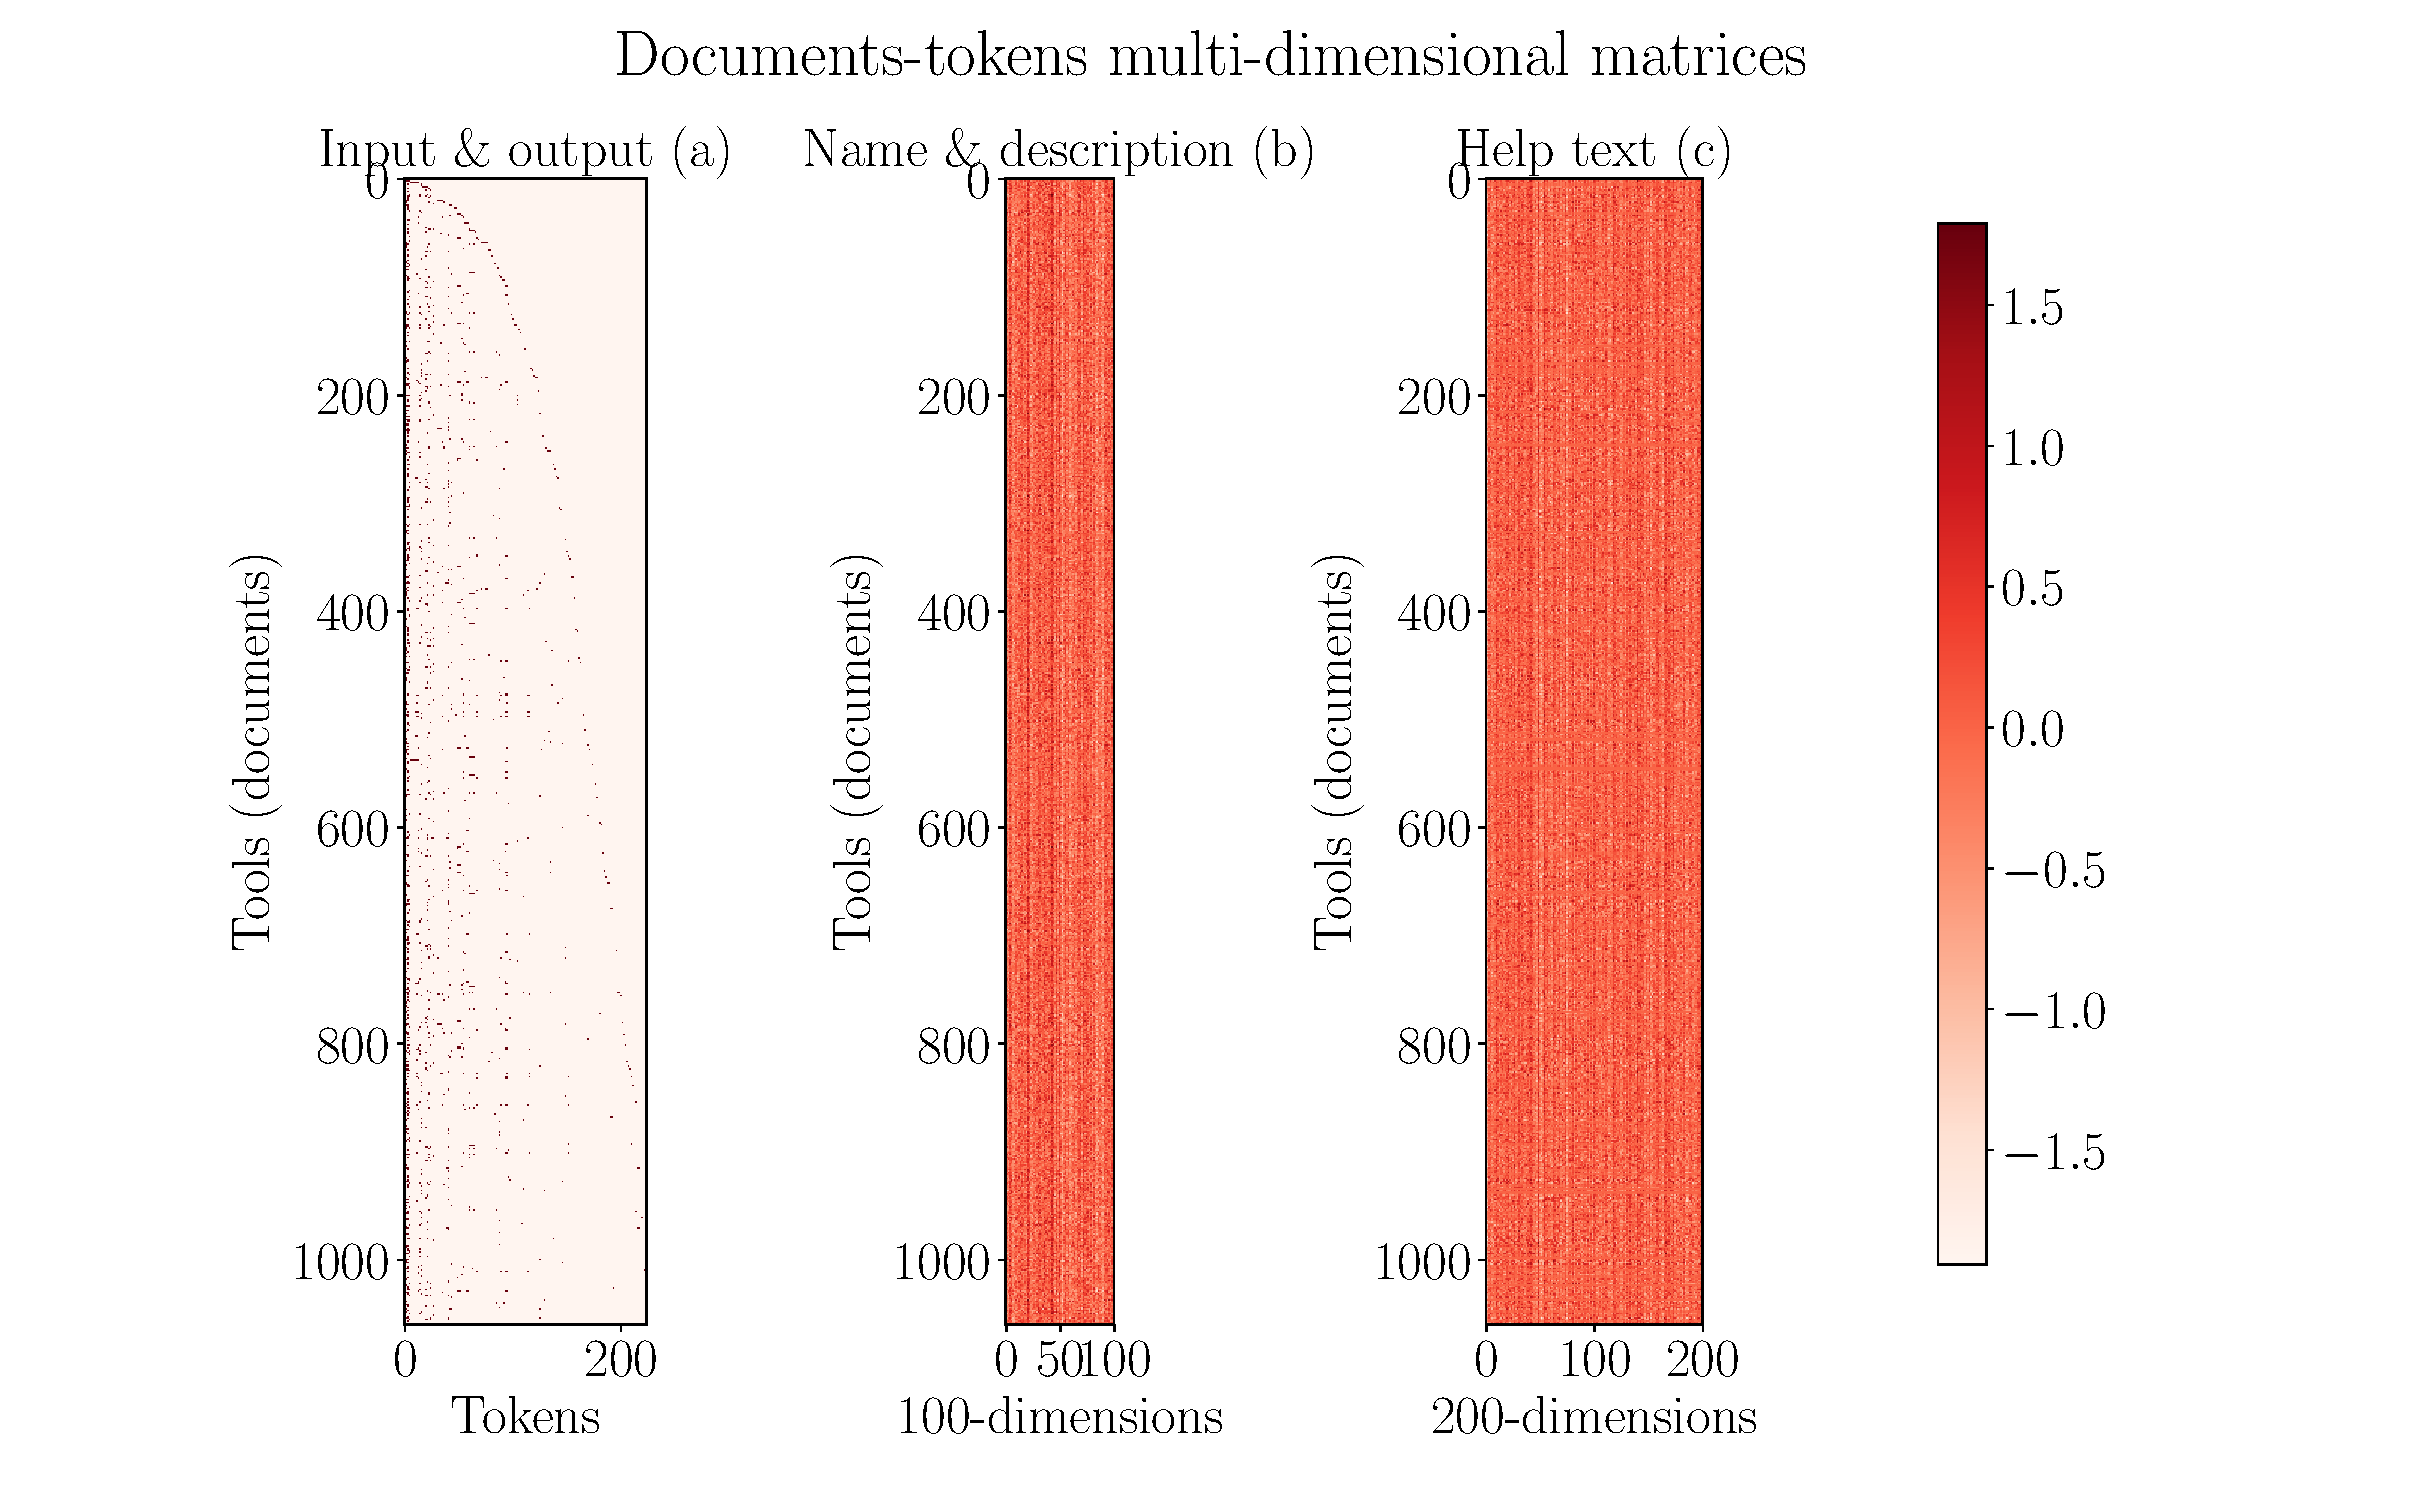
\includegraphics[scale=0.35]{figures/Documents-tokens_doc2vec.pdf}}
    \caption[Documents-tokens matrices for paragraph vectors]{\textbf{Documents-tokens matrices for paragraph vectors approach}: The heatmap shows documents-tokens matrices for input and output file types (a), name and description (b) and help text (c) attributes. The matrix in (a) is a document-token matrix where each entry shows a relative frequency of the token's occurrence. The matrices in (b) and (c) are 100 and 200 dimensional (each row is a document vector) respectively which means that each row of a matrix belongs to a document (paragraph) and is fixed-length and dense in nature. }
\end{centering}
\end{figure}

\begin{figure}[h]
\begin{centering}    
    {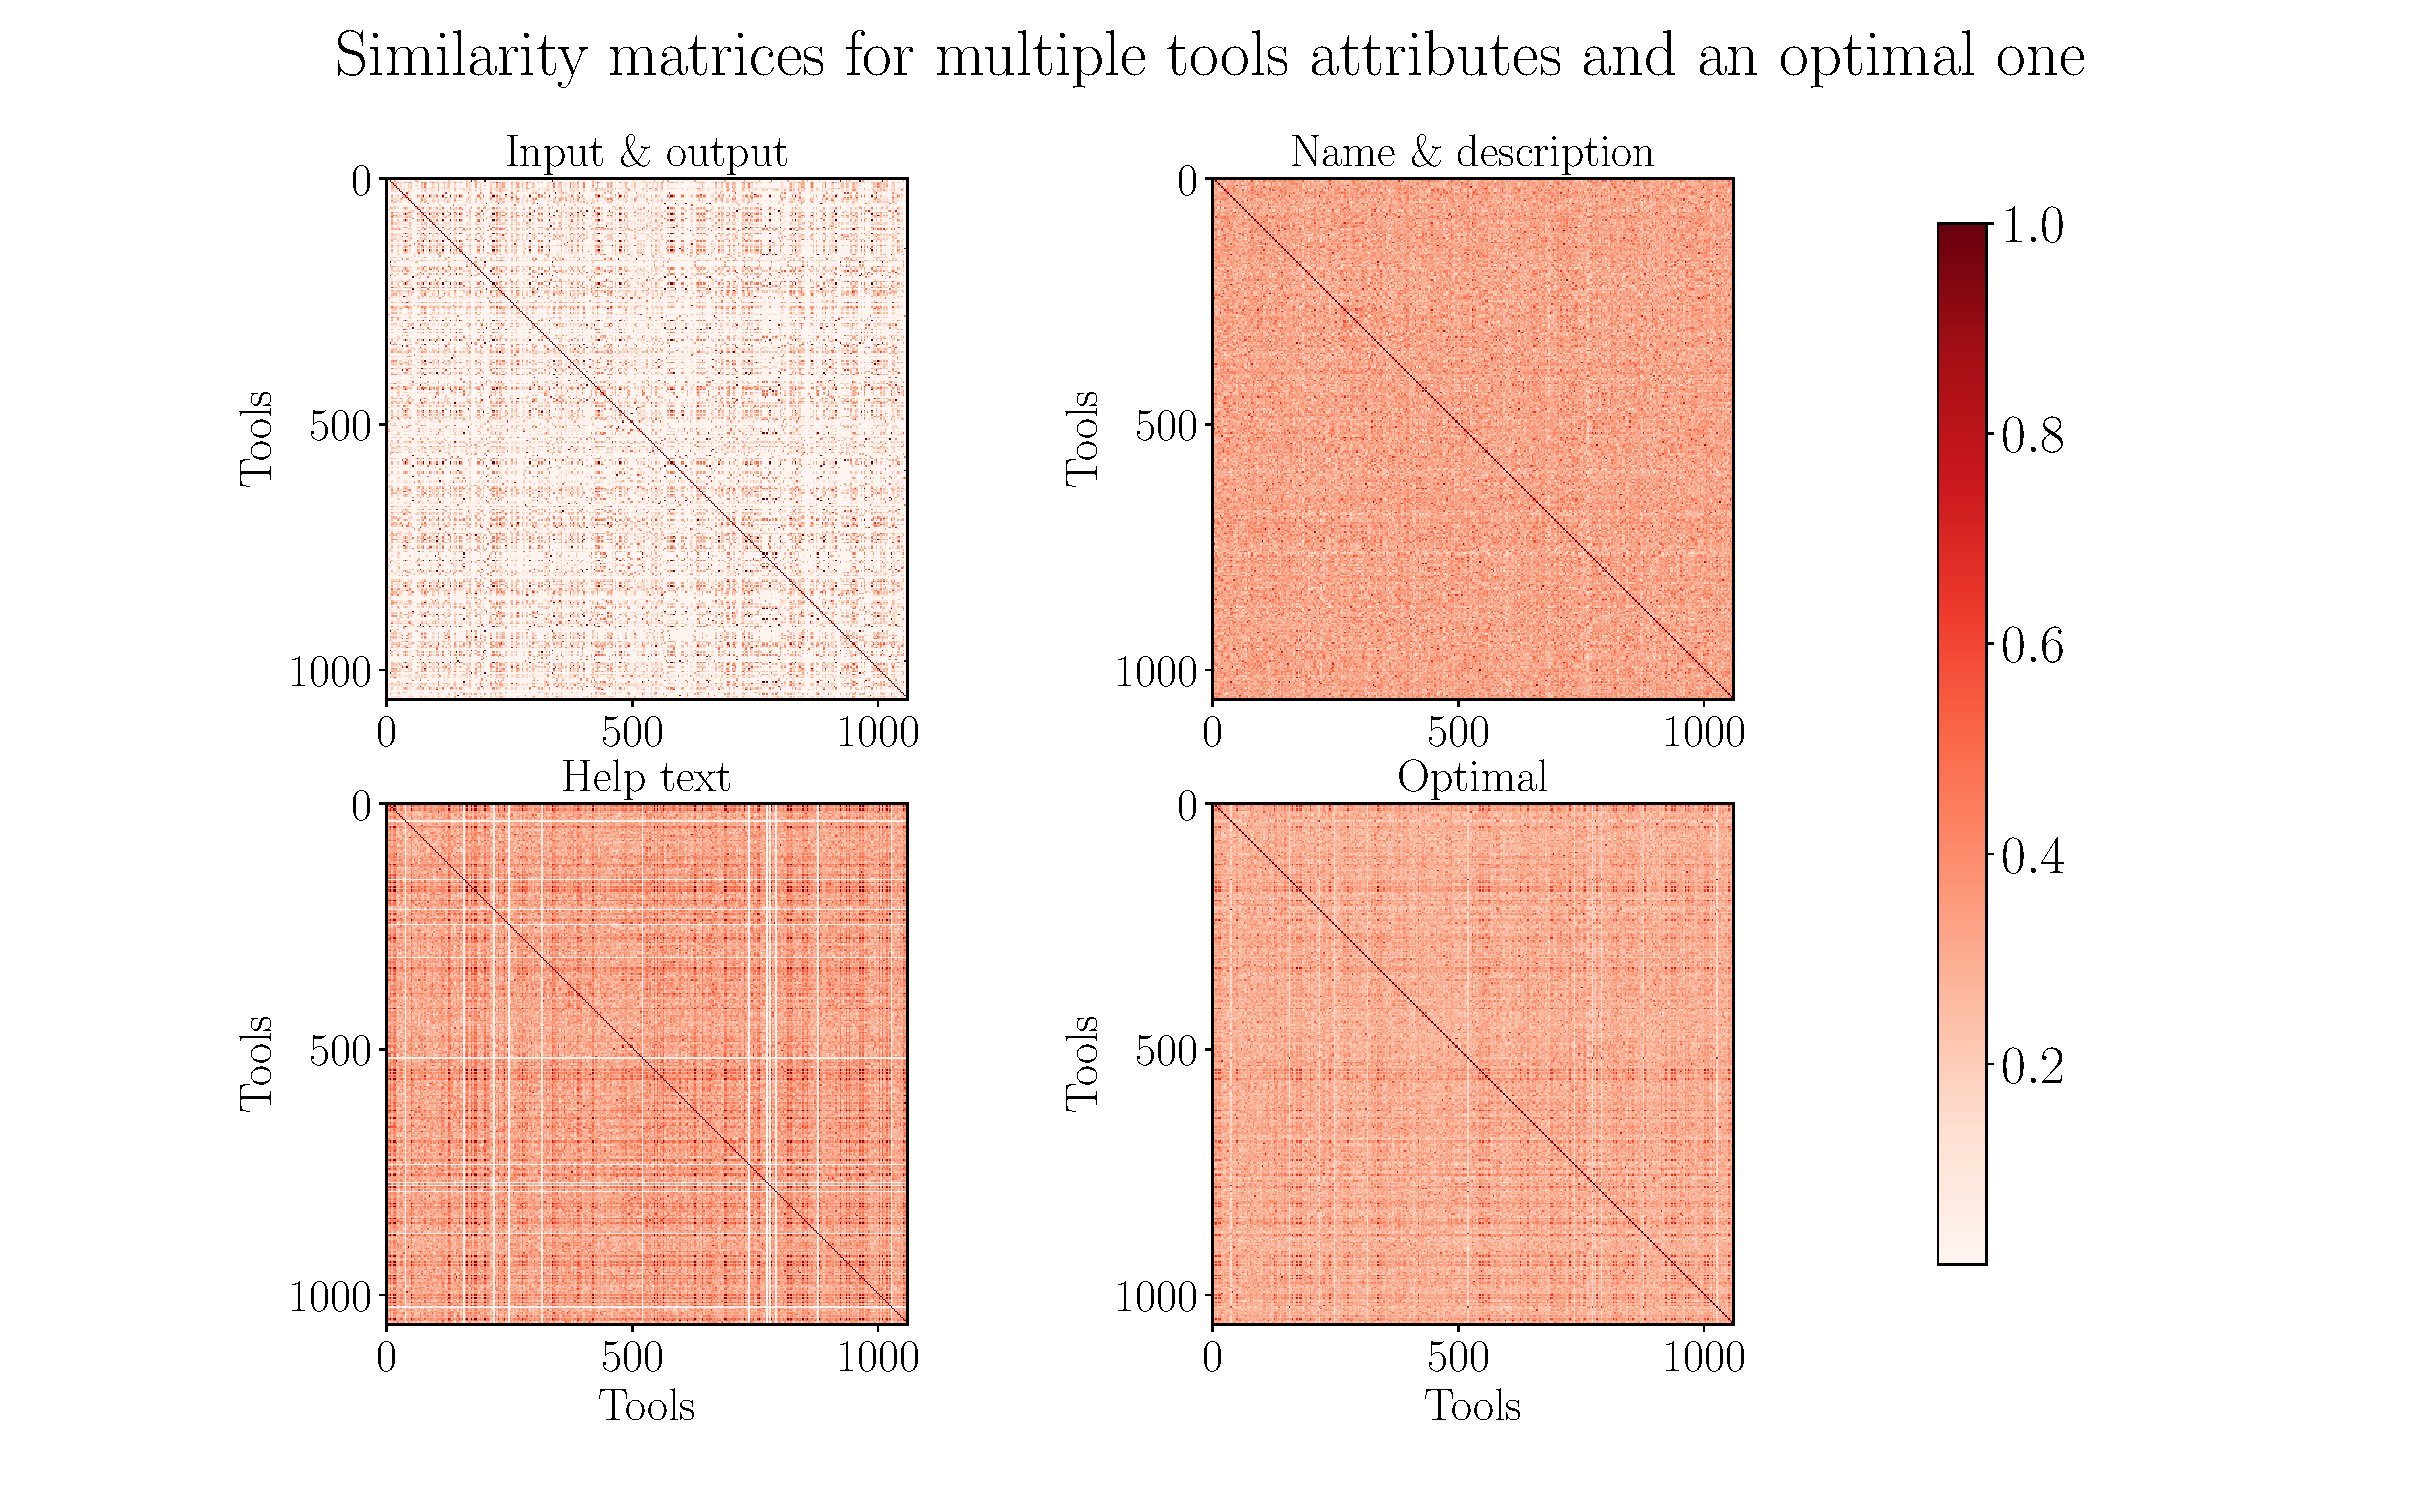
\includegraphics[scale=0.35]{figures/Similarity_matrices_doc2vec.pdf}}
    \caption[Similarity matrices using paragraph vectors approach]{\textbf{Similarity matrices using paragraph vectors approach}: The heatmap shows documents-documents (tools-tools) correlation matrices for input and output (a), name and description (b) and help text (c) attributes. The (d) shows a documents-documents (tools-tools) correlation matrix which is the weighted average computed using (a), (b) and (c) and weights (figure 22) given by the gradient descent optimizer (equation 15). The corresponding documents-tokens matrices are computed as shown in figure 26.}
\end{centering}
\end{figure}

\begin{figure}[h]
\begin{centering}
    {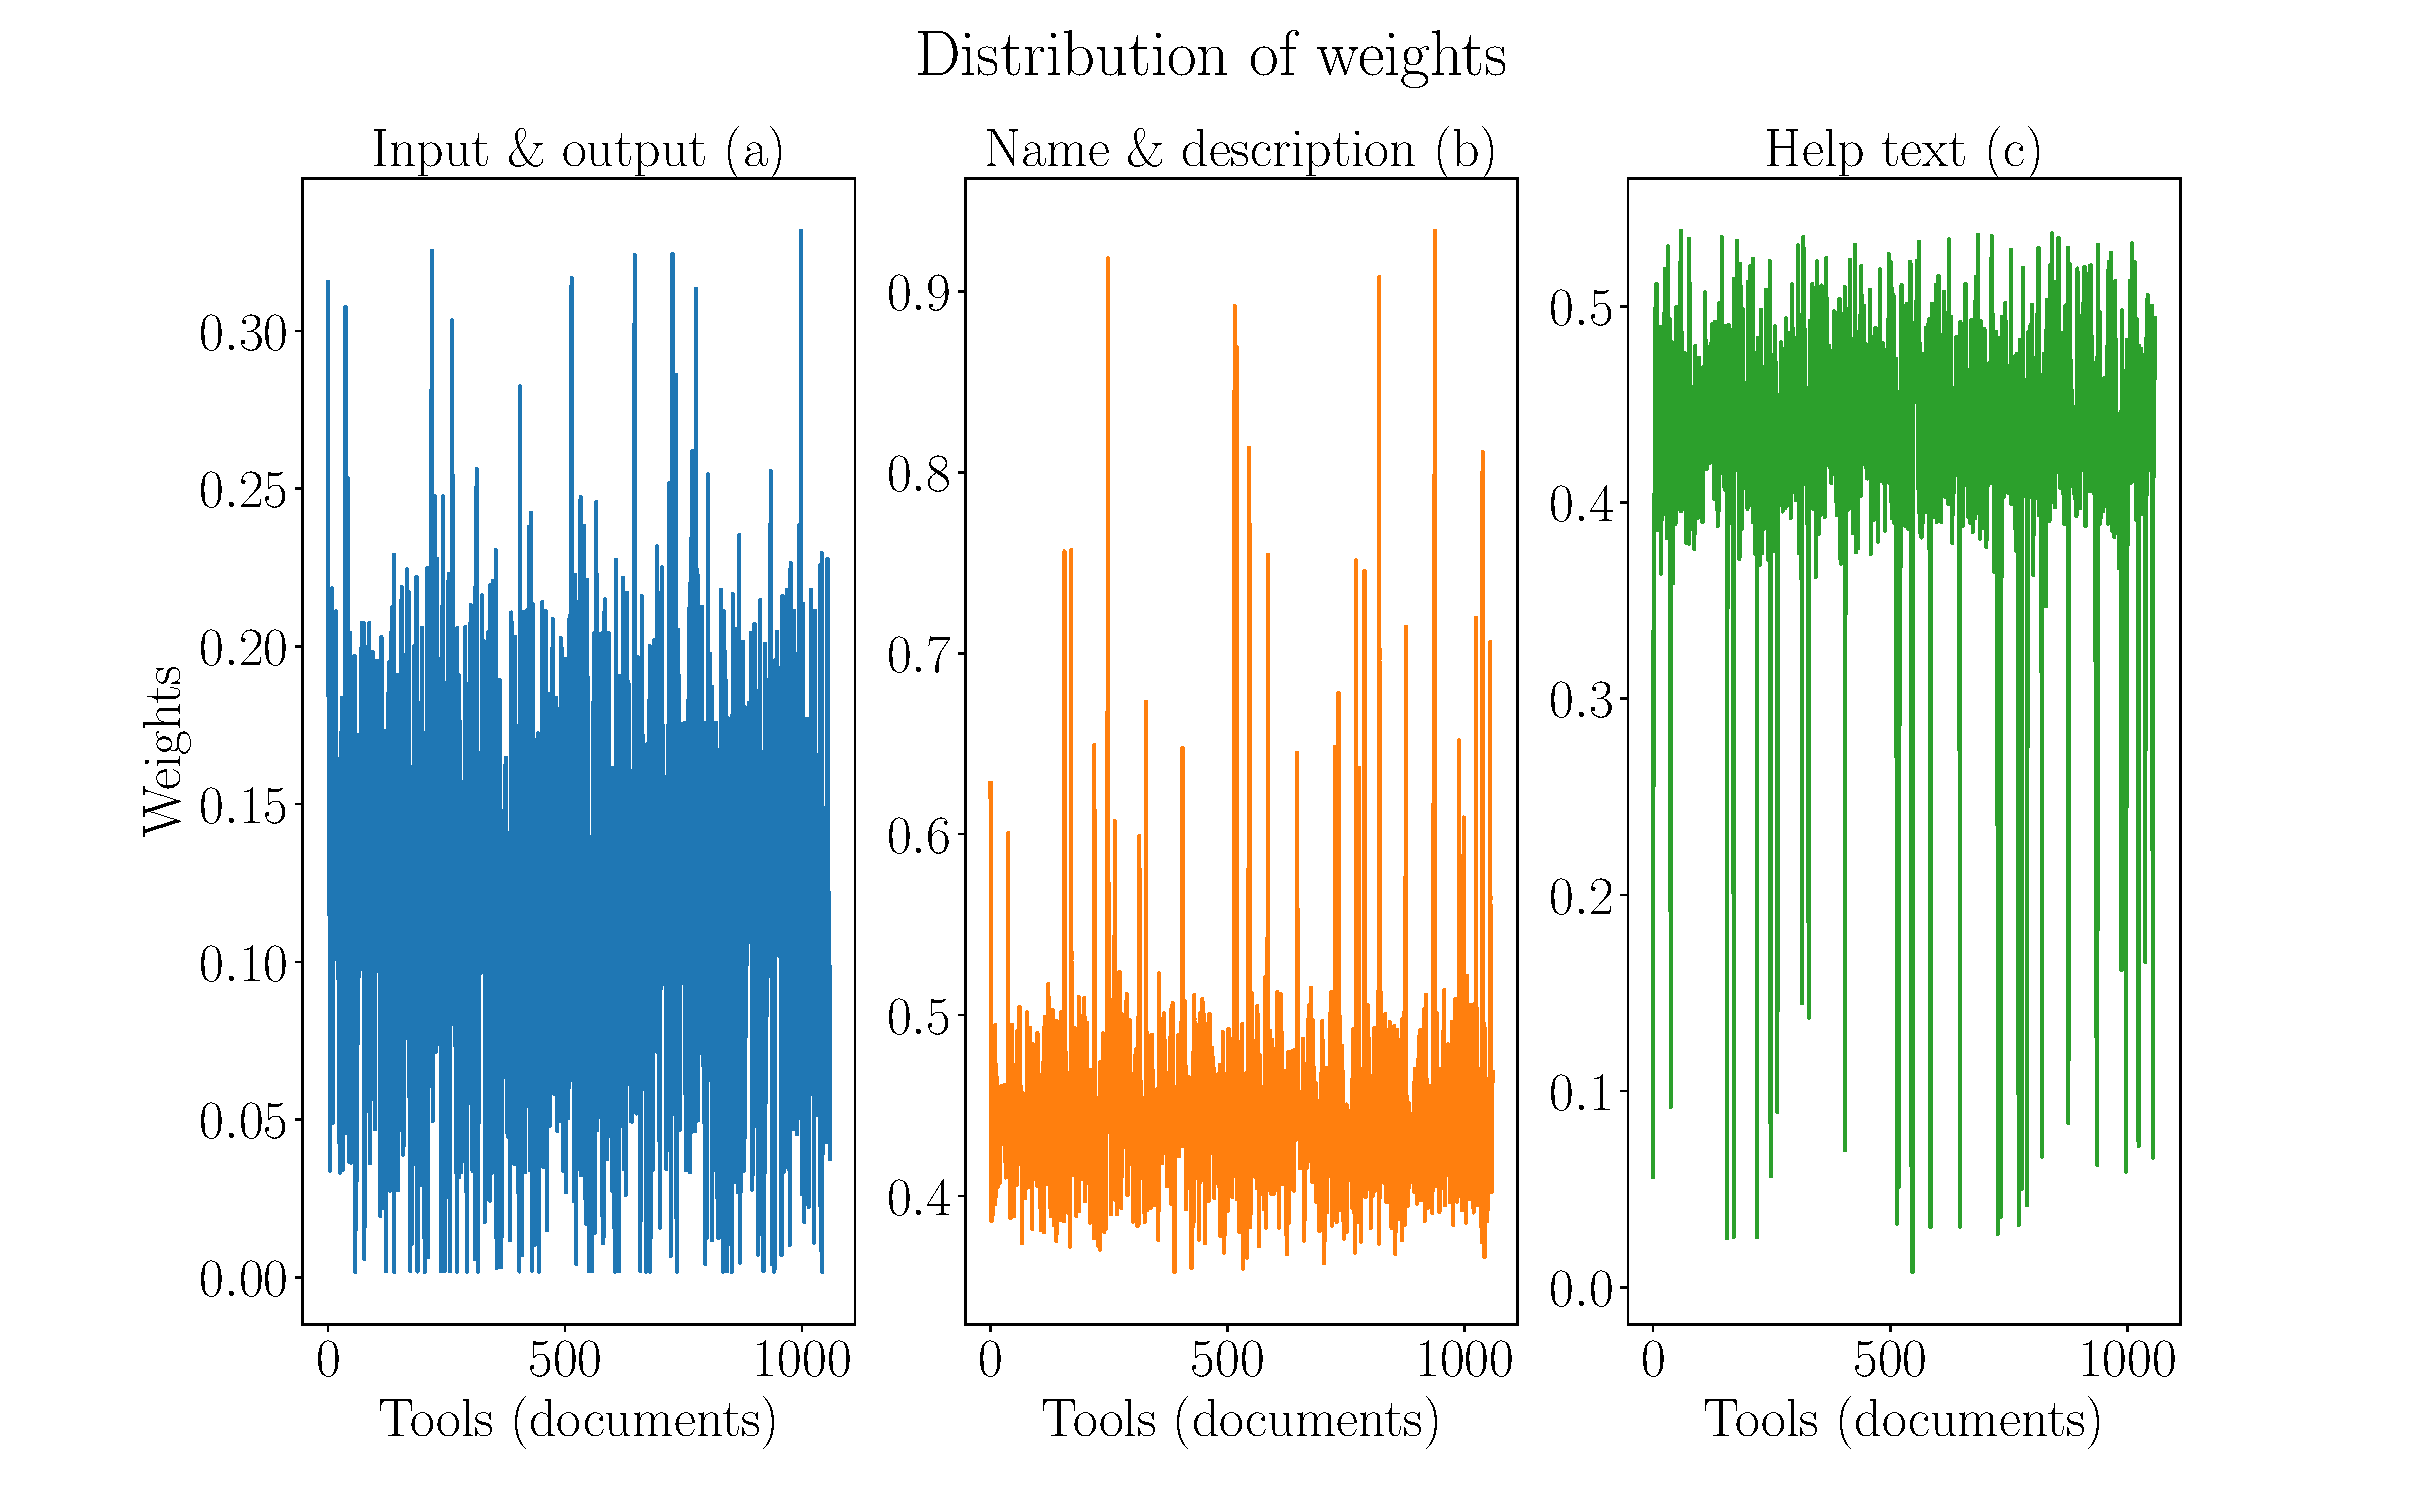
\includegraphics[scale=0.35]{figures/Weights_doc2vec.pdf}}
    \caption[Weights distribution for doc2vec]{\textbf{Weight distribution learnt using paragraph vectors approach}: The plot shows the distribution of weights learned by gradient descent optimizer on the similarity matrices for the input and output (a), name and description (b) and help text (c) attributes. The corresponding documents-tokens matrices are computed as shown in figure 26. }
\end{centering}
\end{figure}

\subsection{Optimization}
\begin{figure}[h]
\begin{centering}
    {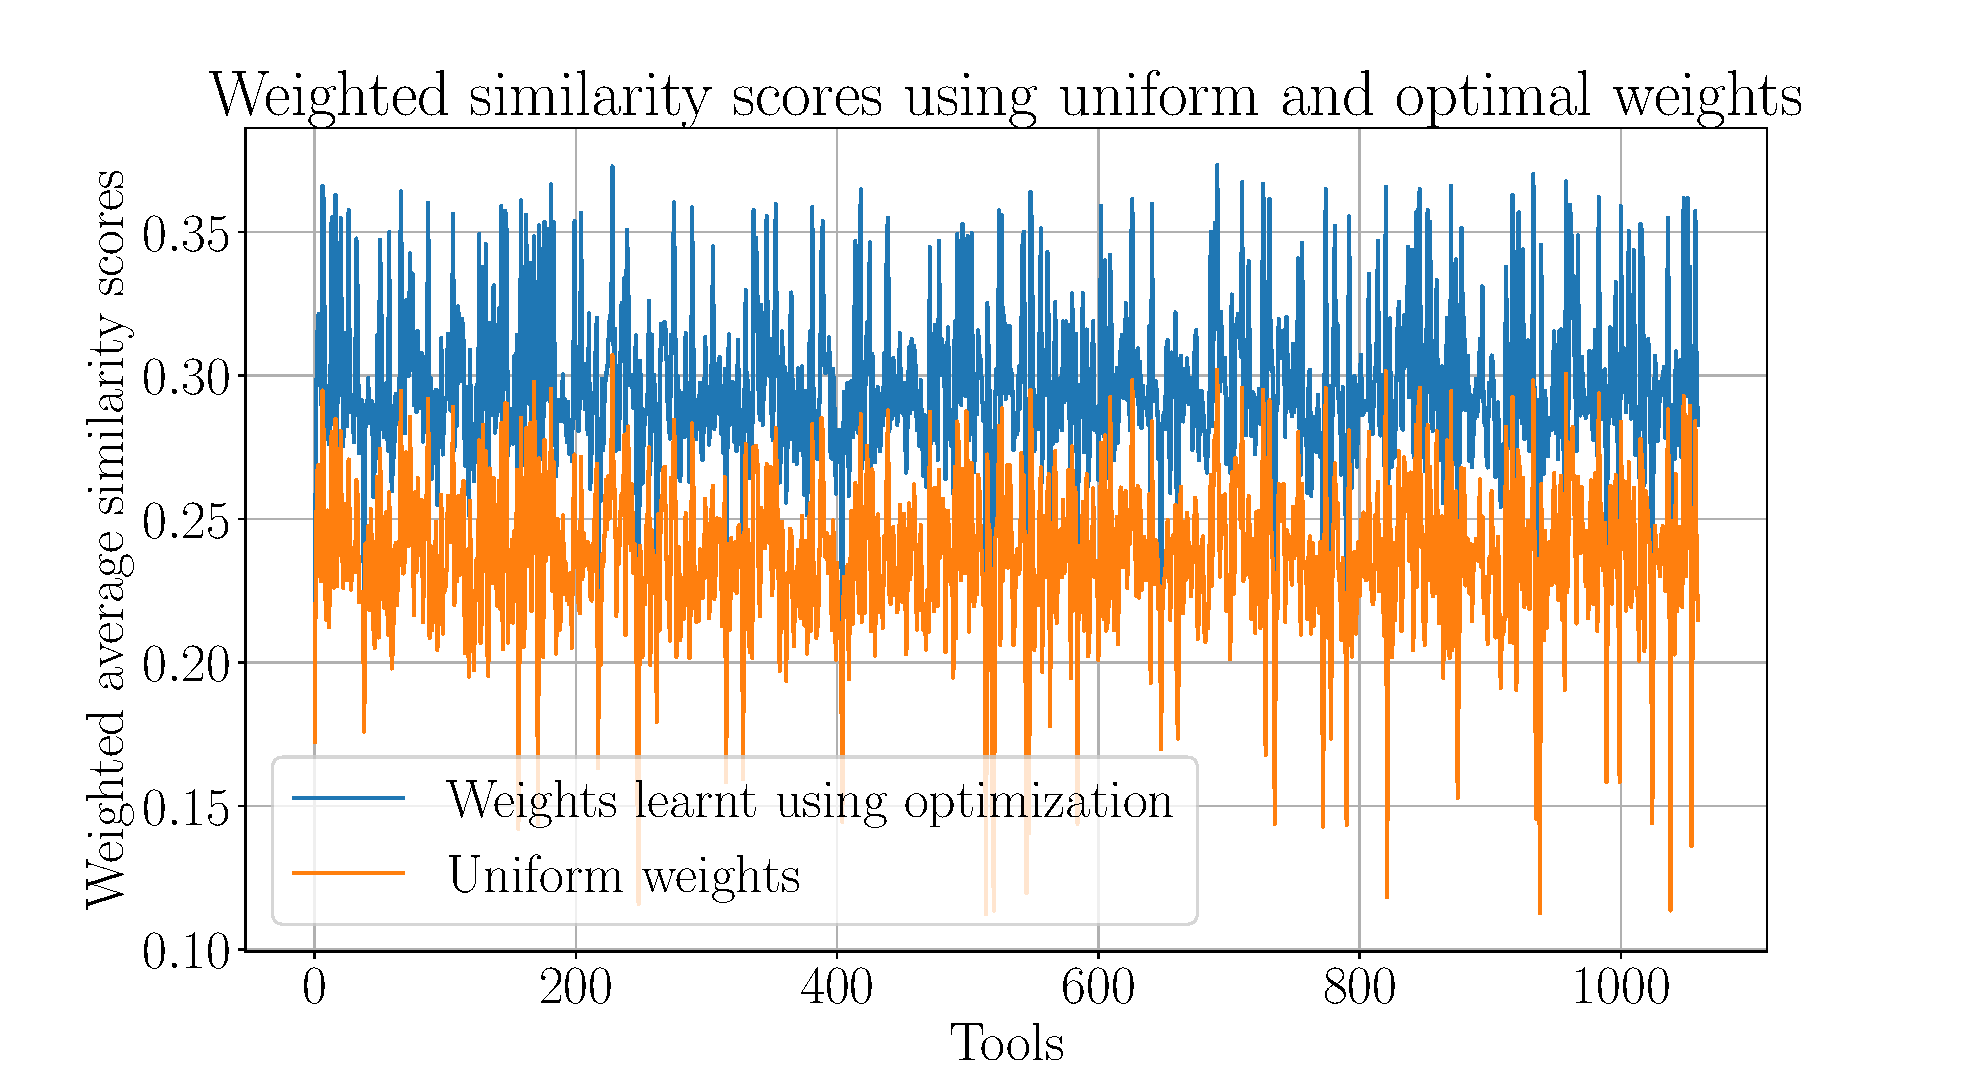
\includegraphics[scale=0.45]{figures/weighted_optimal_uniform_scores.pdf}}
    \caption[Optimal uniform similarity scores]{\textbf{Similarity scores learned using optimal and uniform weights for paragraph vectors approach}: The plot shows a comparison of average similarity scores computed across all tools using weights learned using optimization and uniform weights. }
\end{centering}
\end{figure}


\subsection{Visualizer for paragraph vectors approach}
% screenshots


